%%%%%%%%%%%%%%%%%%%%%%%%%%%%%%%%%%%%%%%%
% Classe do documento
%%%%%%%%%%%%%%%%%%%%%%%%%%%%%%%%%%%%%%%%

% Nós usamos a classe "unb-cic".  Deixe apenas uma das linhas
% abaixo não-comentada, dependendo se você for do bacharelado ou
% da licenciatura.

\documentclass[bacharelado]{unb-cic}
%\documentclass[licenciatura]{unb-cic}



%%%%%%%%%%%%%%%%%%%%%%%%%%%%%%%%%%%%%%%%
% Pacotes importados
%%%%%%%%%%%%%%%%%%%%%%%%%%%%%%%%%%%%%%%%

\usepackage[brazil,american]{babel}
\usepackage[T1]{fontenc}
\usepackage{indentfirst}
\usepackage{natbib}
\usepackage{xcolor,graphicx,url}
\usepackage[utf8]{inputenc}
\usepackage{amsmath}
\usepackage{graphicx}
\usepackage{url}
\usepackage{algorithm}
\usepackage{algorithmic}

%%%%%%%%%%%%%%%%%%%%%%%%%%%%%%%%%%%%%%%%
% Cores dos links
%%%%%%%%%%%%%%%%%%%%%%%%%%%%%%%%%%%%%%%%

% Veja o arquivos cores.tex se quiser ver que outras cores estão
% pré-definidas.  Utilizando o comando \hypersetup abaixo nós
% evitamos aquelas caixas vermelhas feias em volta dos links.

%%%%%%%%%%%%%%%%%%%%%%%%%%%%%%%%%%%%%%%%
% Cores do estilo Tango
%%%%%%%%%%%%%%%%%%%%%%%%%%%%%%%%%%%%%%%%

\definecolor{LightButter}{rgb}{0.98,0.91,0.31}
\definecolor{LightOrange}{rgb}{0.98,0.68,0.24}
\definecolor{LightChocolate}{rgb}{0.91,0.72,0.43}
\definecolor{LightChameleon}{rgb}{0.54,0.88,0.20}
\definecolor{LightSkyBlue}{rgb}{0.45,0.62,0.81}
\definecolor{LightPlum}{rgb}{0.68,0.50,0.66}
\definecolor{LightScarletRed}{rgb}{0.93,0.16,0.16}
\definecolor{Butter}{rgb}{0.93,0.86,0.25}
\definecolor{Orange}{rgb}{0.96,0.47,0.00}
\definecolor{Chocolate}{rgb}{0.75,0.49,0.07}
\definecolor{Chameleon}{rgb}{0.45,0.82,0.09}
\definecolor{SkyBlue}{rgb}{0.20,0.39,0.64}
\definecolor{Plum}{rgb}{0.46,0.31,0.48}
\definecolor{ScarletRed}{rgb}{0.80,0.00,0.00}
\definecolor{DarkButter}{rgb}{0.77,0.62,0.00}
\definecolor{DarkOrange}{rgb}{0.80,0.36,0.00}
\definecolor{DarkChocolate}{rgb}{0.56,0.35,0.01}
\definecolor{DarkChameleon}{rgb}{0.30,0.60,0.02}
\definecolor{DarkSkyBlue}{rgb}{0.12,0.29,0.53}
\definecolor{DarkPlum}{rgb}{0.36,0.21,0.40}
\definecolor{DarkScarletRed}{rgb}{0.64,0.00,0.00}
\definecolor{Aluminium1}{rgb}{0.93,0.93,0.92}
\definecolor{Aluminium2}{rgb}{0.82,0.84,0.81}
\definecolor{Aluminium3}{rgb}{0.73,0.74,0.71}
\definecolor{Aluminium4}{rgb}{0.53,0.54,0.52}
\definecolor{Aluminium5}{rgb}{0.33,0.34,0.32}
\definecolor{Aluminium6}{rgb}{0.18,0.20,0.21}

\hypersetup{
  colorlinks=true,
  linkcolor=DarkScarletRed,
  citecolor=DarkScarletRed,
  filecolor=DarkScarletRed,
  urlcolor= DarkScarletRed
}



%%%%%%%%%%%%%%%%%%%%%%%%%%%%%%%%%%%%%%%%
% Informações sobre a monografia
%%%%%%%%%%%%%%%%%%%%%%%%%%%%%%%%%%%%%%%%

\title{Earthquake Risk Induction Models with Evolutionary Computation}

\orientador{\prof \dr Marcelo Ladeira}{CIC/UnB}
\coorientador{\prof \dr Claus de Castro Aranha}{Department of Computer Sciences/University of Tsukuba}
\coordenador{\prof \dr Homero Luiz Piccolo}{CIC/UnB}
\diamesano{20}{dezembro}{2013}

\membrobanca{\prof \dr Claus de Castro Aranha}{Department of Computer Sciences/University of Tsukuba}
\membrobanca{\prof \dr Guilherme Novaes Ramos}{CIC/UnB}

\autor{Yuri Cossich}{Lavinas}
\CDU{004.4}

\palavraschave{algoritmos genéticos, sismos, terremotos, log-likelihood}
\keywords{genetic algorithms, earthquake, log-likelihood}



%%%%%%%%%%%%%%%%%%%%%%%%%%%%%%%%%%%%%%%%
% Texto
%%%%%%%%%%%%%%%%%%%%%%%%%%%%%%%%%%%%%%%%

\begin{document}
  \maketitle
  \pretextual

  \begin{agradecimentos}
  to be done
  \end{agradecimentos}
\selectlanguage{brazil}
  \begin{resumo}
  Enteder os mecanismos e padrões dos terremotos é imporatnte para minimizar suas consequências. Neste contexto, este projeto visa desenvolver um modelo de previsão de riscos de terremotos com Computação Evolutiva (EC). O objetivo principal é definir um método para estumar a probabilidade de ocorrências de terremotos no Japão usando dados históricos de terremotos para uma determinada região geográfica. Este trabalho se baseia no contexto do  “Collaboratory for the Study of Earthquake Predictability” (CSEP), que visa padronizar os estudos e testes de modelos de previsão de terremotos. O método é baseado em uma apliacação de Algoritmos Genéticos (GA) e busca desenvolver um método estatístico de análise de risco de terremotos. Os modelos de risco gerados por esta aplicação foram analisados pelos valores obtidos de {\it log-likelihood}, como sugerido pelo {\it Regional Earthquake Likelihood Model} (RELM). Os modelos são comparados com os dados reais e com os modelos gerados pelo método do {\it Relative Intensity Algorithm} (RI). Os dados utilizados foram obtidos da {\it Japan Metereological Angency} (JMA) e são relativos à atividades sísmicas no Japão entre os anos de 2000 e 2010.
  \end{resumo}

  \selectlanguage{american}
  \begin{abstract}	
To understand the mechanisms and patterns of the earthquakes is very important to minimize its consequences. In this context, this projects aims to develop an earthquake prevision risk model using Evolutionary Computation (EC). The main goal is to define a method to estimate the probability of earthquake occurrences in Japan using historical earthquake data of a given geographical region. This work is established in the context of the “Collaboratory for the Study of Earthquake Predictability” (CSEP), which seeks to standardize the studies and tests of earthquake prevision models. The method is based in one application of Genetic Algorithms (GA) and aims to develop statistical methods of analysis of earthquake risk. The risk models generated by this application were analyzed by their log-likelihood values, as suggested by the Regional Earthquake Likelihood Model (RELM). They are compared with real data and the models generated by the application of the Relative Intensity Algorithm (RI). The data used was obtained from the Japan Metereological Angency (JMA) and are related with earthquake activity in Japan between the years of 2000 and 2010.

Earthquake Risk Models describe the risk of occurence of seismic
events on a given area based on information such as past earthquakes
in nearby regions, and the seismic properties of the area under study. 
These models can be used to 


Recently, Evolutionary Computation has been used to learn risk models
using purely past earthquake occurrence as training data. While the
results were promising, we believe that a much better model could be
learned if domain knowledge, such as known theories and models on
earthquake distribution, were incorporated into the Evolutionary
Algorithm's training process.

In this work we approach this idea by improving former methods in two
ways: (1) We modify the genome representation of a model from an
area-based representation to an earthquake representation, and (2) we
use known methods from seismology (such as the Omori-Utsu formula) to 
refine the candidates generated by the GA.

We analyze the contributions from each of these modifications using
the methodologies described in the Collaboratory for The Study of
Earthquake Predictability (CSEP), and compare their performance with
(XXX method and YYY method). Our results indicate that (XXX result,
YYY result)

  \end{abstract}
  \selectlanguage{american}

  \tableofcontents
  \listoffigures
  \listoftables

  \textual
  \chapter{Introduction}
In this chapter we present a general specification of the problem, its relevance and what are the goals of this study.

\section{Earthquakes}
Earthquakes may cause lots of damages environment and consequently may represent, directly or inderectly, a risk to human lives. They manifest themselves by shaking and sometimes displacement of the ground. They may also cause tsunamis, landslides, volcano activities, etc.\\

%TODO: explain aftershock
%TODO: i may need to add references of the quakes
There are many examples that show how devastating one large earthquake can be. In April 2015,there was a magnitude 7.8 $M_w$ earthquake in Nepal. It cause 8000 deaths and triggered two avalanches, one of them in the Mount Everest. Also, many people were made homeless, it destroyed UNESCO World Heritage sites and had many aftershocks, including a magnitude $M_w$ 7.3 quake that caused 200 deaths. Another example happened in March 2011, Japan. It was a 9.0 $M_w$ earthquake, and it is considered the most powerful earthquake to ever hit Japan and the 4th most powerful in the world. It caused tsunami waves that reached more than 40 meters, moved the main island in Japan more than 2 meters east and also changed the Earth axis. It was reported that it caused more than 15000 deaths, made more than 200000 people homeless and provoked a meltdown of the Fukushima Daiichi Nuclear Power Plant complex. (see Figure 1.1 for a picture of the devastation) (May i use this picture?). Also in 2011 a magnitude $M_w$ 7.1 earthquake hit Van,Turkey and caused lots of deaths and great damages.These are only three very recent examples of large earthquake damages of how dangerous earthquakes can be.\\

Those earthquakes, and many others that hazard the human society, have some common characteristics. They not only are powerful quakes but they happened nearby populated areas, which increase the damaged provoked. To minimize as much as possible future earthquake disaster, a lot can be done. That include to developing goos urban planings, for example to build structures with techniques that can withstand the forces of earthquakes, to create earthquake warning systems, to create more precise civil enginnering codes, and such.\\

To be able to prevent as many casualty as possible, we need the patterns and mechanisms behind the occurrence of earthquakes. We need to know if there is any relationship between the earhquake locations and its time of occurrance, how they are related to each other, et cetera. With this information, it is possible to to create better seismic risk forecast models, indicating which regions show a higher probability of earthquake occurrence at certain periods in time. \\

Until by now, it has been difficult to clearly understand the many different seismic variables (hours, magnitude, local, depth,...) influences the quakes and either exists a mathemathical model capable of supplying detailed and precise information about the relations and ways to estimate them. Therefore, to develop a prediction earthquake model can prove itself very complex.\\

\section{Earthquake Prediction}

Earthquake prediction is a polemic subject. No research has even come close to suggesting that individual large scale earthquakes can be predicted~\cite{ecta14} and many scientists think that earthquake prediction may not be fully impossible but that the resources needed for such a prediction may be out of reach~\cite{eberhard2014multiscale}.\\

%TODO: check the nature1999 
In the context of this study, we do not aim to predict any individual earthquake and its major characteristics. Our goal relies on the fact that earthquakes do cluster in time and space. We want to use computer techniques to learn and to generate risk models. There is a lot of value behind the study of earthquake mechanisms, with the goal of generating statistical models of earthquake risk~\cite{Nature1999}.\\

In~\cite{Koza2003}, Koza says that Evolutionary Computation (EC) may find, by try trial and error, based on a great amount of data, better solutions for problems that human beings may not find it easy to solve. EC is a family of subfield of artificial intelligence that aim to extract patterns and to solve problems using a great amount of data, by trial and error.We may also say that without any domain knowl- edge about the problem to be controlled, the EC learns about it by trial and error~\cite{Michie94machinelearning}.\

%TODO": what are black box problems?
EC are based on methaheuristic or stochastic optimization, and are mostly applied for black box problems. They are interesting to be used specially in cases that are difficult to understand and the knowledge available is not sufficiently available.\\

Based on these information and on the difficulty to understand how earthquakes behave, we want to explore historical earthquake data using EC. It is expected that it will help to find new ideas about earthquakes, their patterns and their mechanisms behind each earthquake occurrence. For doing so, we need first to outline the forecast problem, then verify the suitability of Evolutionary Computation to the problem of generating earthquake forecast models.\\

Next, we will study ways to improve the generated methods using both EC and other computer techniques and any siesmological knowledge. For this phase we want to propose different representations aiming to refire the algorithm performance and to incorporate seismology methods to refine the models proposed.\\


%\section{Objetivos}
%Este trabalho visa construir um modelo baseado em dados históricos para estimar ocorrência de sismos utilizando dados reais obtido pela {\it Japan Metereological Agency} (JMA). O modelo gera indivíduos que são possíveis soluções para o problema e os indivíduos de cada população são avaliados pela função de {\it fitness} que utiliza testes sugeridos pela {\it Study of Earthquake Predictability} (CSEP).\\
%
%O objetivo principal do trabalho é mostrar que criar um modelo de previsão de terremotos desenvolvido a partir de Computação Evolutiva é possível e promissor, como também garantir uma qualidade do modelo perante outros modelos de previsão de riscos. %Esperamos atrair mais atenção para futuras pesquisas nessa área.
%%arrumar aqui 
%

  %\chapter{The Earthquake Forecasting Problem}~\label{chapter2}
This chapter focus on the theoretical concepts used as base for this study. The main topics are the CSEP framework and its tests.\\

\section{Earthquake Likelihood Model Testing}~\label{testing}

We started studies of the earthquake forecasting problem by determining and selecting ways to build earthquake forecast models, to evaluate and to compare them, as suggested by the Collaboratory for the Study of Earthquake Predictability (CSEP). It is an international partnership to promote rigorous study of the feasibility of earthquake forecasting and predictability~\cite{ecta14}.\\

For that, we gathered some important information about earthquake predicting needed for this study. Most of it is based on the paper {\it Earthquake Likelihood Model Testing} \cite{schorlemmer2007earthquake}. From this paper we gathered information that guided us into how to build, evaluate and compare earthquake forecast models efficiently.\\

A very difficult and yet very common problem when studying earthquake models is how to compare different kinds of models, that are based on different tests protocols. The CSEP proposes a methodology for rigorous scientific testing of these many different models. This group proposed an framework called The CSEP framework. It provides a method to compare earthquakes risk models in an objectively and consistently way~\cite{ecta14}.\\

All forecast models proposed in this study are based in the Collaboratory for the Study of Earthquake Predictability (CSEP) framework. In the CSEP framework, a forecast model uses a gridded rate forecast \cite{zechar2010evaluating}, one common format in the literature. For evaluate and compare these models we used the likelihood based tests. They are the L-test, the N-test and the R-test, as suggested by Regional Earthquake Likelihood Model (RELM)~\cite{schorlemmer2007earthquake}.\\

%TODO: rewrite this
The principle behind each consistency test is the same. One calculates a goodness-of-fit statistic for the forecast and the observed data. One then estimates the distribution of
this statistic assuming that the forecast is the data-generating model (by simulating catalogues that are consistent with the forecast). One then compares the calculated statistic with the estimated distribution; if the calculated statistic falls in lower tail of the estimated distribution, this implies that the observation is inconsistent with the forecast, or that the forecast should be “rejected”. For the CSEP consistency tests used here, the likelihood is the fundamental metric, but this approach would be similar for different statistical measurements~\cite{eberhard2014multiscale}.\\

\subsection{Vector of expectations}~\label{vector}
As stated in section~\ref{testing}, The CSEP framework uses a gridded rate forecast. This gridded forecast may be structured by a vector of earthquake expectations, occurrences probabilities, that are directly related to a vector of real earthquake observations.\\

Based on this structure, it is possible to calculate the Log-likelihood value of a model with the real data observed. It is also possible to use comparison tests based on the calculation of the Log-likelihood.\\

\subsection{The Log-Likelihood Function}\label{log-fuction}
%All the methods use the log-likelihood value for the fitness function. The fittest individual among all the others, is preserved in the next generation, to make the solution of one generation as good as the its last generation.a gene of the genome representation 
To calculate the Log-likelihood value we need both vectors cited above, in section~\ref{vector}. One of them is the vector of earthquake expectations and the other is the vector of real earthquake observations. On them, each element is considered a bin. \\

Each bin, $b_n$, define the set $\beta$ and $n$ is the size of the set $\beta$:
\begin{equation} 
\beta := {b_1,b_2,...,b_n},n = |\beta|.
\end{equation}
The probability values of the model $j$, expressed by the symbol
$\Lambda$, is made of expectations $\lambda_i^j$ by bin $b_i$. The
vector is define as:
				
\begin{equation}
	\Lambda^j = 
\begin{pmatrix}
    \lambda_1^j, 
    \lambda_2^j, 
    \hdots,
    \lambda_i^j
  \end{pmatrix}
  ;\lambda_i^j := \lambda_i^j(b_i),b_i \in \beta
\end{equation}
		
The vector of earthquake quantity expectations is defined as:
earthquake by time. The $\Omega$ vector is composed by observations
$\omega_i$ per bin $b_i$, as the $\Lambda$ vector:

\begin{equation}
\Omega = 
\begin{pmatrix}
    \omega_1,
    \omega_2,
    \hdots,
    \omega_i
  \end{pmatrix}
  ;\omega_i =\omega_i(b_i),b_i \in \beta
\end{equation}

The calculation of the log-likelihood value for the $\omega_i$
observation with a given expectation $\lambda$ is defined as:


\begin{equation}
	L(\omega_i|\lambda_i^j) = -\lambda_i^j + \omega_i\log\lambda_i^j - \log\omega_i!
\end{equation}

The joint probability is the product of the likelihood of each bin, so
the logarithm $L(\Omega|\Lambda^j)$ is the sum of for
$L(\omega_i|\lambda_i^j)$ every bin $b_i$:

\begin{equation}\label{log-like}
\begin{split}
	L^j = L(\Omega|\Lambda^j) = \sum_{i=1}^{n}L(\omega_i|\lambda_i^j)  \\
	= \sum_{i=1}^{n} -\lambda_i^j + \omega_i\log\lambda_i^j - \log\omega_i!  
\end{split}
\end{equation}

The fitness function is a coded version of the equation
~\ref{log-like}. It uses the probabilities of the bins of each
individual of model for the $\lambda$ values.\\
				
\subsection{Uncertainties in Earthquake Parameters}
It is important to say that the earthquake parameters, as the location, magnitude and focal time, cannot be estimated without uncertainties. Therefore, each parameter uncertainty has to be included in the testing~\cite{schorlemmer2007earthquake}. Moreover, by estimating it, it is possible to judge the reliability and robustness of the forecast testing~\cite{eberhard2014multiscale}. Also, each observation must be treated as independent ones. This is not the case of the aftershocks, once they are directly dependent with another stronger earthquake. \\

\section{Tests for evaluating Models}\label{Tests}
In the paper {\it Earthquake Likelihood Model Testing}~\cite{schorlemmer2007earthquake}, it is proposed some statistical tests that are used in this study, developed by the The
Regional Earthquake Likelihood Models (RELM). They were used to compare
and evaluate the every forecast models. These tests are based on the
log-likelihood score that compares the probability of the model with
the observed events.\\

To evaluate the data-consistency of the forecast models we used the
N-Test, the Number Test, and the L-Test, or Likelihood Test. These
tests fall are significance tests. Therefore, assuming a given forecast
model as the null hypotheses, the distribution of an observable test
is simulated. If the observed test statistic falls into the upper or
lower tail of this distribution, the forecast is
rejected~\cite{schorlemmer2010first}.\\

To be able to compare the model that passed the N-Test and the L-test,
the R-Test, the hypotheses Comparison Test, is used. It calculates the
relative performance of a model, by comparing the Log-likelihood
values between two forecast models.\\
%TODO: zechar files format
\subsection{L-test - Data-consistency test}\label{Ltest}
The L(ikelihood)-Test considers that the likelihood value of the model
is consistent with the value obtain with the simulations. The value is
calculated by fowling the formula, where $\widehat{L}_k$ is the value of the
Log-likelihood of the model {\it j}, in the {\it bin} {\it i} and
$\widetilde{L}$ is the value of the Log-likelihood of the simulation
{\it j} in the {\it bin} {\it q}:


\begin{equation}
\gamma^{j}_{q} = \frac{\left| \left\{ \widehat{L}^j_k | \widehat{L}^j_k \leq \widetilde{L}^j_q, \widehat{L}^j_k \in \widehat{L}^j, \widetilde{L}^j_q \in \widetilde{L}^j  \right\} \right|}  {|\widehat{L}^j|}
\end{equation}

The analysis of the results can be splitted into 3 categories, as follows:

\begin{enumerate}
\item Case 1: $\gamma^{j}$ is a low value, or in other words, the
  Log-likelihood of the model is lower then most of the Log-likelihood
  of the simulations. In this case, the model is rejected.
\item Case 2: $\gamma^{j}$ falls near the half of the values obtained
  from the simulations and is consistent with the data.
\item Case 3: $\gamma^{j}$ is high. This means that the Log-likelihood
  of the data is higher that the Log-likelihood of the model and no
  conclusion can be made what so ever.
\end{enumerate}


It is important to highlight that no model should be reject in case 3,
if based only on the L-Test. In this case the consistency can or
cannot be real, therefore these model should be tested by the N-Test
so that further conclusions can be done.\\

\subsection{Number test or N-Test}
The N(umber)-Test also analyses the consistency of the model, but it
compares the number of observations with the number of events of the
simulations. This test is necessary to supply the under predicting
problem, which may pass unnoticed by the L-Test.\\

This measure is estimated by the fraction of the total number of
observations by the total number of observations of the model.\\

As the L-test, if the number of events falls near the half of the
values of the distribution, then the model is consistent with the
observation, nor estimating too much events nor too few of them.\\

\subsection{Hypotheses Comparison Test or R-Test}

The Hypotheses Comparison, or the R(atio)-Test, compares two forecast
models against themselves. The log-likelihood is calculated for both
models and then the difference between them is calculated, named the
observed likelihood ratio. This value indicates which one of the model
better fits the observations.\\

The likelihood ratio is calculated for each simulated catalogue If the
fraction of simulated likelihood ratios less than the observed
likelihood ratio is very small, the model is reject.  To make this
test impartial, not given an advantage to any model, this procedure is
applied symmetrically~\cite{schorlemmer2010first}.\\


\subsection{Evaluation}\label{eval}
This section may need to be placed elsewhere.

The evaluation process is made as follow: First, the data-consistency
is tested by the L-Test and R-test. If the model passes these
tests, meaning that it was not rejected by them, they are compared
with other forecast models, which were also not reject, with the
R-Test. The model that best fits the R-Test is then chose as the best
model~\cite{schorlemmer2007earthquake}.\\

  %TODO: get some info from descricaoDetalhada
\chapter{Models}~\label{chapter3}
As stated in the Section \ref{testing}, all forecast models proposed for this study are based in the Collaboratory for the Study of Earthquake Predictability (CSEP) framework.\\

We propose four forecast model methods. The main difference between them is that they have different genome representation. The genome for each forecast model focus on different aspects of the framework, therefore their represantion vary.\\

The first method is the GAModel~\cite{ecta14}, a statistical method of analysis of
earthquakes risk using the Genetic Algorithm technique (GA). It is a straight application of the CSEP framework. The next method is a specialization of GAModel. It focuses only on areas on which earthquakes happened already in a near past. This will lead to a faster convergence, once the amount of parameters is smaller and consequently, the search space gets smaller. We called it ReducedGAModel(bad name? suggestions?). These methods useonly computational algorithms and techniques.\\

Another method is the Emp-GAModel (bad name? suggestions?). This method incorpores some
geophysical knowledge. It is a hybridization of the models generated by the GAModel with some empirical laws that will be discussed further, in Section \ref{m+a+e}. We also applied these empirical laws in the ReducedGAModel, and name it Emp-ReducedGAModel.\\

%TODO: realocate to->???
For all methods, the population is evolved taking into account earthquake event data for a training period, which is anterior to the target test period. After completing the evaluation stop criteria, the best individual is chosen to be the representative forecast model for that method.\\

\section{1-year Forecast Models}\label{1year-model}
Based on the gridded rate forecast explained in the last Chapter~\ref{chapter2}, we developed earthquake forecasts methods that will estimate the risk of earthquakes occurrence to a target region, during a time interval. Some of the methods also may estime the magnitude of these shocks. For this study we considered the target time interval of one year~\cite{ecta14}.\\

There is no physical measurement to identify mainshocks and its aftershocks~\cite{schorlemmer2010first}, we divided the forecast models in two classes: the ones that only forecasts mainshocks, using only GA techniques, and those that forecast both mainshocks and aftershocks using both GA techniques and empirical laws, such as the modified Omori law. These laws are use to derive the aftershocks from a sintetic data of mainshocks.\\

%TODO: explain better what mainshock and aftershock are
Mainshocks are large and independent earthquakes. They are followed by a wave of others earthquakes, the aftershocks~\cite{schorlemmer2010first}.\\

\section{Mainshock Methods}\label{mainshocksMethods}
The mainshock methods are considered as methods to generate space-rate-time forecasts. They could be described as:

\begin{equation}\label{gamodel}
 \Lambda(t,x,y,M|\Upsilon_t) = \mu(x,y)
\end{equation}

where the number of earthquakes forecast in all bins can denoted as $\Lambda(t,x,y)$~\cite{zechar2010evaluating} given that $\Upsilon_t$ is the earthquake observation data up to time $t$.\\

\subsection{GAModel}\label{GAModel}
The GAModel is completely based on the framework suggested by the CSEP. In it, one forecast is defined as a region in a specfic time interval and is divided in bins. Each bin represents a geographical interval. The whole target area of study is covered by a group of these bins where each bin has an earthquake forecast value. This groups of bin represent the $\mu(x,y)$, the background intensity~\cite{zhuang2004analyzing}. In the GAModel, each possible solution is represented as an entire forecast model.\\

The GAModel forecasts only earthquakes with magnitude greater than 3.0, for every scenario proposed. The space interval for the magnitude is 0.1, named as cells. That results in magnitude cells of [3.0, 3.1), [3.1, 3.2), until [9.9, 10).\\

\subsubsection{Genome Representation}\label{genomeGA}
In the GAModel each individual represents an entire forecast model. Each gene of the individual is a real value, corresponding to one bin in the desired model. The values are sampled from the interval [0, 1). These real values are converted to a integer forecast, we use the same modification of the Poisson deviates extraction algorithm~\ref{inversePoisson} used in~\cite{ecta14}. In the algorithm $x$ is the real value that will be converted and $\mu$ is the mean of the earthquakes observations in the real data. \\

\begin{algorithm}\label{inversePoisson}
  \caption{Obtain a Poisson deviate from a $[0,1)$ value}
  \label{InversePoisson}
  \begin{algorithmic}
    \STATE Parameters $0 \leq x < 1, \mu \geq 0$
    \STATE $L \gets \exp{(-\mu)}, k \gets 0, prob \gets 1$
    \REPEAT 
    \STATE $\text{increment }k$
    \STATE $prob \gets prob*x$
    \UNTIL{$prob > L$}
    \RETURN $k$
  \end{algorithmic}
\end{algorithm}

The genome is a real valued array X, where each element corresponds to one bin in the desired model (the number of bins n is defined by the problem). Each element $x_i \in X$ takes a value from $[0,1)$. In the initial population, these values are sampled from a uniform distribution and they are randomly generated. For more details of the genome representation, please refer to~\cite{ecta14}.\\


To clarify how the GAModel works, we use the same example as the one used in~\cite{ecta14}. The "Kanto" region, one of the four areas used in both studies, is divided into 2025 bins (a grid of 45x45 squares). Each bin has an area of approximately $25km^2$. The GAModel then calculates an expected number of earthquakes for every bin on a determinated time interval, so the GA searches for good values in 2025 bins.\\
\subsubsection{Fitness Function}\label{fitGA}

To compare the indididual data with the observated data, we use the log-likelihood calculation as fitness function. This equation allow us to compare events in the observated data with the values of occorrences obtained by a model. The models that have more similarity with to the observated data have bigger log-likelihood values. The fittest individual among all the others, is preserved inthe next generation, to make the solution of one generation as good as the its last generation.\\

The fitness function is a coded version of the equation ~\ref{log-fuction}. It uses the probabilities of the bins of each individual of model for the $\lambda$ values.\\

\subsubsection{Evolutionary Operators}\label{gaOperators}
The GAModel use a combination of operators made available by the Distributed Evolutionary Algorithms in Python (DEAP)~\cite{DeRainville:2012:DPF:2330784.2330799}. We used the One Point Crossover for the crossover operator, the Polynomial Bounded Mutation for the mutation operator and for selection, we used Tournament selection and Elitism. The parameters are described in the Table~\ref{GAParameters}.

\begin{table}[!ht]
  \caption{Parameters used in GAModel and Emp-GAModel}
  \label{GAParameters}
  \begin{center}
  \begin{tabular}{|l|r|}
    \hline
    Population Size & 500\\
    Generation Number & 100\\
    Elite Size & 1\\
    Tournament Size & 3\\
    Crossover Chance & 0.9\\
    Mutation Chance (individual) & 0.1\\
	Polynomial Bounded parameters & eta = 1, low = 0, up = 1\\
    \hline    
  \end{tabular}
  \end{center}
\end{table}

%TODO: put this under!
The parameters of the Polynomial Bounded mutation funcition are: add online ref???
\begin{enumerate}
\item eta = 1. Crowding degree of the mutation. A high eta will produce a mutant resembling its parent, while a small eta will produce a solution much more different;
\item o low = 0. The lower bound of the search space;
\item o up = 1. The upper bound of the search space.
\end{enumerate}

The chance of applying both mutation operator function and crossover operator function takes into account only their chance of occurrence. This means that it may be the case that one of them or both are not applied.\\

\subsection{ReducedGAModel}\label{ReducedGAModel}
The GAModel defines a expected number of earthquakes for every single bin in the target region. That could lead to exhaustive and, sometimes worthless, searches. That is caused by the number of bins in the forecast and also because in some bins there are no earthquake occurances in the observation data. That means that the GAModel has a lot of parameters and may of its bins have null values (values igual to 0). To avoid such unnecessary task we proposed the ReducedGAModel.\\

With this method, we aim to minimize the search space and the quantity of parameters the GA has to deal with. For that we changed the individual representation. The individuals in the ReducedGAModel only define expected number of earthquakes in bins that already had some occurance in the past, giving a direction to where the GA should search. That helps the ReducedGAModel in the search for better solutions and it makes the convergence faster once the space search is smaller.\\

The ReducedGAModel has a similar description of the GAModel. As said in the last paragraph, the difference is that, in the ReducedGAModel, each possible solution represents only a fraction of the forecast where we expect to find especific risk areas. To do so, this method will obtain the position of past occurances. Then it will calculate some expected number of earthquakes only for the bins related to those positions. These positions may vary during the evoluting of the method, including positions that never had earthquake events before. That is important to add some variation to the method.\\

The ReducedGAModel, as the GAModel~\ref{GAModel}, forecasts only earthquakes with magnitude greater than 3.0, for every scenario proposed. The space interval for the magnitude is 0.1, named as cells. That results in magnitude cells of [3.0, 3.1), [3.1, 3.2), until [9.9, 10).\\

\subsubsection{Genome Representation}\label{genomeReduced}
The genome representation in the ReducedGAModel is a simplified version of the genome of the GAModel. For the ReducedGAModel, the genome is a list of ordered pairs. The first element of the pair are the coordenates of a bin in the model. The second element of the pair is a number that indicates an earthquake occurrence estimative for this bin.\\

%TODO: explain this better
To calculate the size of the individual we use the real data from the pior 5 years and create a list of every bin that had events in it, even if only once.\\

In the ReducedGAModel, each individual is a list of a subregion of the forecast model. This list initially refers to bins where earthquake events happened in the past. During the develop of the ReducedGAModel, the list may refer to positions that never had occurrences before. Each element of the list, a gene, also contains one real value between [0,1). In the initial population, these values are sampled from a uniform distribution and they are randomly generated. When needed, every real value is converted to a integer forecast by the algorithm~\ref{inversePoisson}, as in the GAModel~\ref{GAModel}.\\

To generate the forecast model we need to do an intermediate step. We map every location from the list with a bin in the forecast model.\\

The genome size is usually smaller than the one used in the GAModel and the Emp-GAModel, once the amount of subregions where earthquakes with magnitude above 3.0 happened for any given area is smaller then the total number of genes of the individual.\\

To examplify, we use a similar example as the one in~\ref{GAModel}. Lets consider that there are 10 bins with occurances in "Kanto" in the last 5 years, it will make the GA start searching for good values for only those 10 bins, leaving the other 2015 bins empty, representing zero occurances. It is important to highlight that in the worst case, it will make the same amount of searches as the GAModel. The final forecast model will maintain the amount of bins with occurrance, but the number of events for every bin and their location may change.\\

\subsubsection{Fitness Function}
The fitness function is the same as in the GAModel,~\ref{fitGA}. Here is also important to generate the forecast model by applying the map function on the individual as in the last Section,~\ref{genomeReduced}.\\

\subsubsection{Evolutionary Operators}\label{ReducedOperators}
All operators in the ReducedGAModel are the same as the operators of the GAModel, except the the mutation fuction. We use a simple mutation operator which samples entirely two new values, both sampled from uniform distributions. The first, is a new real value from [0,1) and the seconde one, a new integer value from [0,$x$), where $x$ is the maximum position value a bin can have in the target region. For the parameters see Table~\ref{GAHParameters}.

\begin{table}[!ht]
  \caption{Parameters used in ReducedGAModel}
  \label{GAHParameters}
  \begin{center}
  \begin{tabular}{|l|r|}
    \hline
    Population Size & 500\\
    Generation Number & 100\\
    Elite Size & 1\\
    Tournament Size & 3\\
    Crossover Chance & 0.9\\
    Mutation Chance (individual) & 0.1\\
    \hline    
  \end{tabular}
  \end{center}
\end{table}

As in the GAModel, see~\ref{gaOperators}, the chance of applying both mutation operator function and crossover operator are independent and they may or may not be used.\\

\section{Mainshock+Aftershock Methods}\label{m+a+e}
%TODO: add the var right values and "faixa"
The mainshock+aftershock methods are a two-step methods. The first step is as defined for the mainshocks methods, therefore, we first use GA techniques to obtain a sintetic mainshock data. The second step is to use seismological empirical equations to obtain the aftershocks from the mainshocks.\\

Hence earthquakes cluster in space and inspired by the space-time epidemic-type aftershock sequence (ETAS), we proposed two methods, called Emp-GAModel and Emp-ReducedGAModel. They represent the ideia of associating the GA with seismological empirical equations. They are described as:

\begin{equation}\label{reducedgamodel}
	\Lambda(t,x,y,M|\Upsilon_t) = \mu(x,y)J(M)
\end{equation}

That can be expanded to:

\begin{equation}\label{emp-model}
 \Lambda(t,x,y|\Upsilon_t) = \mu(x,y) + \displaystyle\sum_{t_i \in t} K(M_i)g(t-t_i)P(x,y)
\end{equation}
%TODO: explicar o Upsilon

The mainshock+afterchock methods use $\mu(x,y)$ as defined for mainshock methods~\ref{mainshocksMethods}. It is calculated as an expected number of earthquakes for every bin in the target region, given that $\Upsilon_t$ is the earthquake observation data up to time $t$.\\\\

The Omori law, $g(t)$, which is considered one empirical formula of great success~\cite{zhuang2004analyzing}\cite{utsu1995centenary}\cite{omori1895after}, is a power law that relates the earthquake occurance and its magnitude
with the decay of aftershocks activity with time. For this approach we used the probabilty density function (pdf) form of the modifed Omori law~\cite{zhuang2004analyzing}:

\begin{equation}\label{omori}
	g(t)= \dfrac{(p-1)}{c(1+ \dfrac{t}{c})^(-p)}
\end{equation}

In the paper~\cite{utsu1995centenary}, Utsu says that most p and c
values, for various earthquake data sets fall in the range between 0.9
and 1.4, and between 0.003 and 0.3 days, respectively. These values
were based on the Davidon-Fletcher-Powell optimization procedure and
used in ETAS~\cite{utsu1995centenary}.\\

Based on paper~\cite{yamanaka1990scaling}, we set the values of $1.3$
for $p$ and $0.003$ for $c$ for our the experiments. Following the
statement make in this report, we set the time interval $t$ between a
mainshock and its aftershocks at one month. The statement says that if
the $t$ value is too short, the number of aftershocks is too small,
but if it is too big, we may also consider background activity.\\

For $K(M_i)$, the total amount of triggered events, we count
aftershocks within a given area, $A$, using the following formula,
where $M_c$ is the magnitude threshold:

\begin{equation}\label{triggered}
 K(M_i) = A\ exp([\alpha(M-M_c)])
\end{equation}

In the paper~\cite{ogata2006space}, it states that $\alpha$ should be
equal to the inverse of the magnitude of an event, or
$magnitide^{-1}$. To obtain $A$, the following equation
from~\cite{yamanaka1990scaling}, was used:

\begin{equation}
A = e^{(1.02M -4)}
\end{equation}

%A partir de K(Mi) e g(t) calculo a quantidade total de aftershocks desencadeados. Faço o somatório do produto das equações, variando t em 0<= t <=30.

\begin{equation}
\displaystyle\sum_{t_i \in t} K(M_i)g(t-t_i)
\end{equation}
% partir do resultado obtido da equação anterior, aplico a distribuição de terremotos pelos bins baseado no RI, a P(x,y).
%P(x,y) pode ser dividido em 4 equações:

and lastly, the $J(M)$ is a simulation of the event magnitude by
Gutenberg-Richter's Law, using Add SAPP\\
% $1$ as the value of $\beta$ ~\cite{helmstetter2003predictability}:
%
%\begin{equation}\label{gut-ritcher}
%J(M) = \beta e^{-\beta(M-M_c)}, M \geq M_c
%\end{equation}

P(x,y) calculates the position of the aftershocks with base on the origin of the mainshock. It is a simple space distribuition function, that alocates the aftershocks in one of the following posotions: upper, lower, left or right. It runs for a number of steps, getting futter from the origin at each step or as when there are no more events to be alocated.\\
%P(x,y) distribui a quantidade de aftershocks obtidos pelo somatório anterior em bins do modelo. Os bins nos quais os afterschoks serão distribuídos são os bins superiores, inferiores e laterais. As variáveis i e j, posições na matriz, são equivalentes a x e y. A variável aftershock é a quantidade de aftershocks relativo a um bin e o decaimento é linear. Row é o comprimento da linha da matriz.\\

\begin{subequations}
\begin{align}
        model[i+j] = (aftershocks-[model[i]-2*i])/4,\\
        model[i-j] = (aftershocks-[model[i]-2*i])/4,\\
        model[i-j*row] = (aftershocks-[model[i]-2*i])/4,\\
        model[i+j*row] = (aftershocks-[model[i]-2*i])/4,
\end{align}
\end{subequations}

\subsection{Emp-GAModel}
The Emp-GAModel is a specialization of the GAmodel. This is achieved by the use of empirical equations after the forecast is provided. This means that the its genome representation are the same as the GAModel.\\
\subsubsection{Genome Representation}
The genome representation is the same as in the GAModel,~\ref{genomeGA}.\\

\subsubsection{Fitness Function}
The fitness function is the same as in the GAModel,~\ref{fitGA}, and the ReducedGAModel.\\
\subsubsection{Evolutionary Operators}
The Emp-GAModel use the same combination of operators that the GAModel. For more explanation, please see~\ref{gaOperators} and table~\ref{GAParameters}.\\

\subsection{Emp-ReducedGAModel}
The Emp-ReducedGAModel is a specialization of the ReducedGAmodel. This is achieved by the use of empirical equations after the forecast is provided. This means that the its genome representation are the same as ReducedGAModel.\\

\subsubsection{Genome Representation}
The genome representation is the same as in the ReducedGAmodel,~\ref{genomeReduced}. \\

\subsubsection{Fitness Function}
The fitness function is the same afor all methods,~\ref{fitGA}. Here is also important to generate the forecast model by applying the map function on the individual as in the last Section,~\ref{genomeReduced}.\\

\subsubsection{Evolutionary Operators}
The Emp-ReducedGAModel use the same combination of operators that the ReducedGAModel. For more explanation, please see~\ref{gaOperators} and table~\ref{ReducedOperators}.\\

\section{Tests for evaluating Models}\label{Tests}

In the paper {\it Earthquake Likelihood Model Testing}~\cite{schorlemmer2007earthquake}, it is proposed some statistical tests that are used in this study, developed by the The Regional Earthquake Likelihood Models (RELM). They were used to compare and evaluate the forecast models. These tests are based on the log-likelihood score that compares the data of a model with the observed data.\\

To evalute the data-consistency of the forecast models we used the N-Test, the Number Test, and the L-Test, or Likelihood Test. These tests fall are significance tests. Therefore, assuming a given forecast model as the null hypothesys, the distribuition of an observable test is simulated. If the observed test statistic falls into the upper or lower tail of this distribuition, the forecast is
rejected~\cite{schorlemmer2010first}.\\

To be able to compare the model that passed the N-Test and the L-test, the R-Test, the hypotheses Comparison Test, is used. It calculates the relative performance of two models, by comparing the Log-likelihood values obtained from them.\\

\subsection{Likelihood Test or L-Test}
 
The L(ikelihood) Test considers that the likelihood value of the model is consistent with the value obtain with the simulations. The value is calculated by the formula, where $\widehat{L}_k$ is the value of the Log-likelihood of the model {\it j}, in the {\it bin} {\it i} and $\widetilde{L}$ is the value of the Log-likelihood of the simulation {\it j} in the {\it bin} {\it q}:


\begin{equation}
\gamma^{j}_{q} = \frac{\left| \left\{ \widehat{L}^j_k | \widehat{L}^j_k \leq \widetilde{L}^j_q, \widehat{L}^j_k \in \widehat{L}^j, \widetilde{L}^j_q \in \widetilde{L}^j  \right\} \right|}  {|\widehat{L}^j|}
\end{equation}

The analisys of the results can be splited into 3 categories, as follows:

\begin{enumerate}
\item Case 1: $\gamma^{j}$ is a low value, or in other words, the
  Log-likelihood of the model is lower then most of the Log-likelihood
  of the simulations. In this case, the model is rejected.
\item Case 2: $\gamma^{j}$ falls near the half of the values obtained
  from the simluations and is consistent with the data.
\item Case 3: $\gamma^{j}$ is high. This means that the Log-likelihood
  of the data da is higher that the Log-likelihood of the model and no
  conclusion can be made what so ever.
\end{enumerate}


It is important to highlight that no model should be reject in case 3, if based only on the L-Test. In this case the consistency can or cannot be real, therefore these model should be tested by the N-Test so that further conclusions can be done.\\

\subsection{Number test or N-Test}
The N(umber)-Test also analises the consistency of the model, but it compares the number os observations with the number of events of the simulations. This test is necessary to supply the underpredicting problem, indicating whether a forecast has predicted too few earthquakes, which may pass unnoticed by the L-Test.\\

This mesure is estimated by the fraction of the total number of observations by the total number of observations of the model.\\

As the L-test, if the number of events falls near the half of the values of the distruition, then the model is consistent with the observation, nor estimating too much events nor too few of them.\\

\subsection{Hypotheses Comparison Test or R-Test}

The Hypotheses Comparison, or the R(atio)-Test, compares two forecast models against themselves. The log-likelihood is calculted for both models and then the difference between them is calculated, named the observed likelihood ratio. This value indicates which one of the model better fits the observations.\\

The likelihood ratio is calculated for each simulated catalog. If the fraction of simulated likelihood ratios less than the observed likelihood ratio is very small, the model is reject.  To make this test impartial, not given an advantage to any model, this procedure is applied symmetrically~\cite{schorlemmer2010first}.\\


\subsection{Evaluation}\label{eval}
The evaluation process is made as follow: First, the data-consitency is tested by the L-Test and the R-test. If the model passes these tests, meaning that it was not rejected by them, they ares compared with other forecast models, which were also not reject, with the R-Test. The model that best fits the R-Test is then chose as the best model~\cite{schorlemmer2007earthquake}.\\

  \chapter{Computação Evolutiva e Previsão de Sismos}~\label{chapter4}
%TODO: get this info from main.pdf
%TODO: update this information
%A relação Computação Evolutiva e Previsão de Sismos ainda é escassa, pouco explorada. Esse capítulo é dedicado a mostrar o que já foi explorado dessa relação pela comunidade acadêmica. \\

O presente capítulo é dedicado a mostrar o que já foi explorado da relação entre Previsão de Sismos e Computação Evolutiva (EC) pela comunidade acadêmica.% Apesar de ser uma relação pouco estudada, a seguir descreveremos trabalhos correlatos.  \\

Uma das abordagens utilizada é a hibridização entre as técnicas de Computação Evolutiva (EC). Zhang e Wang \cite{Zhang2012} utilizaram Algoritmo Genético (GA) para refinar uma Redes Neurais (ANN) e, a partir dessa aplicação, criar um modelo de previsão. Zhou and Zhu \cite{zhou2014earthquake}, para realizar uma previsão da magnitude de sismos, fizeram uma combinação entre ANN e EC.\\

Muitas das aplicações estimam características dos sismos ou de suas atividades, como por exemplo calcular o {\it Peak Ground Acceleration} (PGA), \cite{pga_Kerh, Kermani2009, Cabalar2009}. PGA é uma medida da aceleração do sismo no solo e pode ser utilizada, por exemplo, para projetar estruturas mais resistentes a abalos sísmicos, tendo importância elevada em áreas próximas ao cinturão sísmico \cite{Cabalar2009}.\\

GA já foi utilizado também para decidir a localização, baseado em atividades sísmicas, de estações de sensoriamento no México \cite{Ramos2011}. Ele foi utilizado como uma ferramenta de projeto para construir uma rede de estações em diferentes regiões do México, objetivando formar uma rede com estações em locais ótimos, afim de alertar a população o mais rápido possível para evitar maiores desastres.\\

Já Nicknam \cite{Nicknam2010} e Kennett e Sambrigde \cite{Kennett1992} utilizaram EC para determinar parâmetros para modelos de falhas (como epicentro, localização, profundidade, etc.) de um dado sismo.\\%detalhar mais coisas!!!!!

Huda e Santosa \cite{ijse5762} recentemente publicaram um artigo em que buscam determinar, com algoritmos genéticos, a velocidade das ondas P e S no manto e na crosta terrestres. Ondas P são indicadas como a primeira falha encontrada em dados sismológicos e ondas S são as mudanças causadas na fase das ondas P \cite{ijse5762}. Essa pesquisa busca obter a estrutura do subsolo japonês e, geograficamente, possui o mesmo foco que a presente pesquisa.


In this section we will briefly discuss some reports of the
application of Evolutionary Computation and related method for
Earthquake Risk Analysis.

The usage of Evolutionary Computation in the field of earthquake risk
models is somewhat sporadic. Zhang and Wang~\cite{Zhang2012} used
Genetic Algorithms to fine tune an Artificial Neural Network (ANN) and
use this system to produce a forecast model. Zhou and
Zu~\cite{Feiyan2014} also proposed a combination of ANN and EC, but
their system only forecasts the magnitude parameter of
earthquakes. Sadat, in the paper~\cite{sadat2015application}, follows
the idea oF Zhou and Zu, aiming to predict the magnitude of the
earthquakes in North Iran, but in this case, he used ANN and GA.

Some sismological models were developed aiming to estimate parameter
values by using Evolutionarry Computation. For example, Evolutionary
Computation was used to estimate the peak ground acceleration of
seismically active
areas~\cite{Kermani2009,Cabalar2009,Kerh2010,Kerh2015}. Ramos~\cite{Ramos2011}
used Genetic Algorithms to decide the location of sensing stations and
Saeidian~\cite{saeidian2016evaluation} made a comparation in
performance between the GA and Bees Algorithm to decide which of those
techniques would performe better when chosing the location of sensing
stations. Nicknam et al.~\cite{Nicknam2010} and Kennett and
Sambridge~\cite{Kennett1992} used evolutionary computation to
determine the Fault Model parameters of a earthquake.


%\section{Algoritmos Genéticos – O que são?}

%\subsection{Cálculos}


  \chapter{Análise dos Dados}\label{chapter5}
%TODO: statistical analysis, filtres(?). char, main/afeter shocks, histograms
%pesquisar alguma coisa sobre dados e GA só pra formular uma intro
\section{Dados de sismos}
O foco dessa pesquisa é estudar padrões existentes nas ocorrências de sismos. Para isso é essencial que tenhamos acesso a dados confiáveis, seguros e ricos em detalhes. Pela página da {\it Japan Metereological Agency} fomos capazes de acessar dados fiéis aos nossos interesses. Os dados obtidos são compostos por longitude, latitude, data e horário da ocorrência, magnitude e profundidade. \\
%- JMA\footnote[2]{\url {http://www.jma.go.jp/jma/index.html}}

Para a base de treino, foram separados os sismos considerados mais uniformes, formando o grupo cuja latitude e longitude na superfície representam abalos em áreas terrestres (terremotos), pouco profundos (acima de 20 km de profundidade) e com magnitude acima de 2.5 grau na escala Richter, durante os anos de 2000 a 2013.\\

Para selecionar terremotos, foi preciso extrapolar as informações contidas nos dados e buscar uma forma de, a partir dos dados disponíveis, deduzir quais sismos serão considerados terremotos e quais serão considerados maremotos. Para isso foi utilizamos {\it The Google Elevation API}\footnote[3]{\url {https://developers.google.com/maps/documentation/elevation/?hl=pt-es}}, uma {\it Application Programming Interface} (API) que tem como objetivo fornecer informações sobre todos os locais sobre a superfície terrestre e oceânica. \\

A API foi utilizada por oferecer uma interface HTTP para consulta de dados de elevação territorial, que recebe via url os parâmetros latitude e longitude e retorna, em formato {\it JavaScript Object Notation} (JSON), dados como a altitude relativa à coordenadas fornecidas, dado este necessário para nossos estudos. Os abalos cuja coordenadas na superfície terrestre tivessem altitude relativa ao nível do mar acima de 0.0 foram selecionados.\\

Ao analisar a nova base de treino percebe-se um elevado aumento na quantidade de terremotos em 2011, ano que o terremoto de Tohoku, magnitude 9 na escala Ritcher, ocorreu, Figura \ref{ocorrenciasAno}. Esse terremoto causou aumento desproporcional de sismos em todo o Japão, fato que levou a decisão de limitar a base de treino até o ano de 2010.\\

%pq???
Ainda em relação a base de treino, ela foi alterada para gerar fatias anuais da base de treino anterior, baseadas nos dados cronológicos disponíveis nos dados da JMA. As fatias são definidas da seguinte forma: se a base refere-se a sismos ocorridos em um espaço de 10 anos, a base será divida por 10, gerando fatias anuais (por exemplo, de 2004 até 2005). Dessa forma, espera-se minimizar o {\it overfitting} (super ajustes) a base de dados.\\

{\it Overfitting} é o uso de modelos ou procedimentos que violam parcimônia, isto é, que incluem mais termos que o necessário ou usam abordagens mais complicadas do que necessárias \cite{hawkins2004problem}. Visar minimiza-lo, na aplicação GA, é importante para que tenhamos boas generalizações.\\

Outra limitação imposta a base de dados foi em relação a área analisada. Como buscamos entender os padrões dos sismos, escolhemos quatro regiões do Japão para focar o experimento, Kanto, Kansai, Touhoku e East Japan. A Figura \ref{alljapan} propõe uma visualização dessas regiões no Japão. A seguir descreveremos as quatro regiões.\\

\paragraph{Kanto} Kanto é a região ao redor de Tóquio. É uma área com elevada atividade sísmica durante o período estudado. Essa região foi definida com coordenadas começando em 34.8 Norte, 138.8 Oeste, com  2025 {\it bins}. Cada {\it bin} corresponde a uma área de 25km2.\\

\paragraph{Kansai} Kansai é a região que inclui cidades Kyoto, Osaka e outras. Essa área, ao contrário da região de Kanto, possui uma baixa atividade sísmica. Essa região foi definida com coordenadas começando em 34 Norte, 134.5 Oeste, com  1600 {\it bins}. Cada {\it bin} corresponde a uma área de 25km2.\\

\paragraph{Touhoku} Touhoku é a região definida como a região ao norte da ilha principal japonesa. Ela possui alguns {\it clusters} de atividade sísmicas durante o período estudado. Essa região foi definida com coordenadas começando em 37.8 Norte, 139.8 Oeste, com  800 {\it bins}. Cada {\it bin} corresponde a uma área de 100km2. \\

\paragraph{Leste do Japão} É a região corresponde a costa leste do Japão. Ela se diferencia da área anterior por incluir tanto áreas terrestres como não-terrestres. Foi nessa área que o sismo M9 de 2011 aconteceu. Essa região foi definida com coordenadas começando em 37 Norte, 140 Oeste, com  1600 {\it bins}. Cada {\it bin} corresponde a uma área de 100km2. \\

%\begin{figure}[!htb]
%\centering
%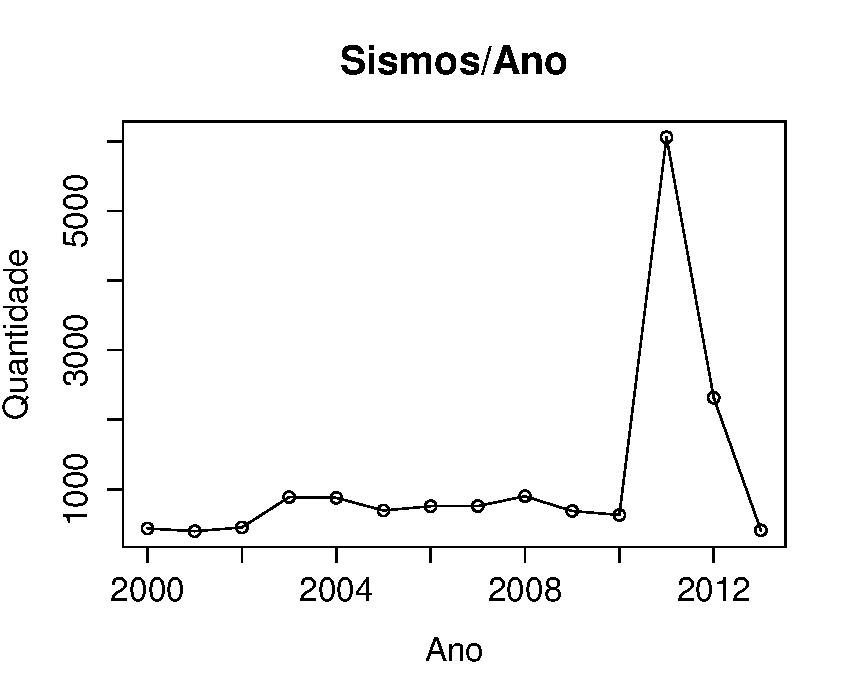
\includegraphics[scale=0.9]{ocorrenciasAno}
%\caption{Quantidade de sismos pelos anos.}
%\label{ocorrenciasAno}
%\end{figure}
%
%\begin{figure}[!htb]
%\centering
%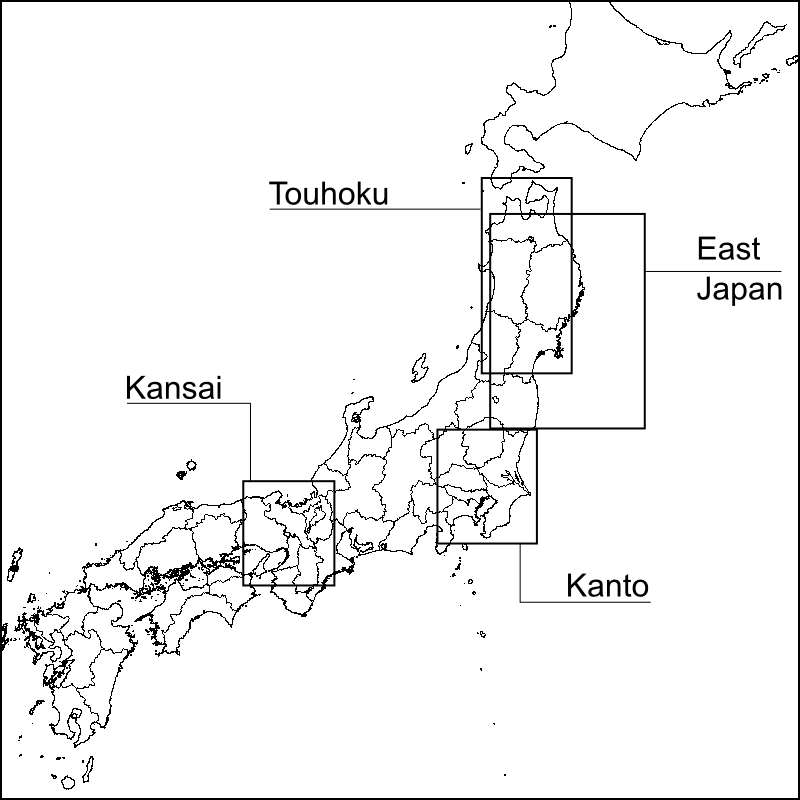
\includegraphics[scale=0.5]{alljapan.png}
%\caption{Áreas priorizadas e suas localização.}
%\label{alljapan}
%\end{figure}



%A última, se refere diretamente a nova base de treino. Ao analizar

1'
  %TODO: add names of the models (gamodel mostly and adequade the params and stuff)
%\chapter{Metodologia Proposta}\label{chapter6}
%TODO: Add section about regions data, move it from the catalog data
%TODO: heat maps
%TODO: boxplot
%TODO: how to produce forecast
%TODO:  how to evaluate
%TODO: add paired test results
\section{Genoma Representation}
Each individual represents an earthquake risk model. It has a number of bins chose to fit the area of study and each bin has a probability value. The areas of study are: Kanto, Kansai, East Japan or Touhoku, see section~\ref{capitulo5}. To obtain the number of earthquakes by the value of the bin, we use the modified Poisson distribution~\cite{NumericalRecipes}.   
	
\begin{algorithm}
  \caption{Obtaining values between $[0,1)$ from the Poissonian curve.}
  \label{InversePoisson}
  \begin{algorithmic}
    \STATE Parameters $0 \leq x < 1, \mu \geq 0$
    \STATE $L \gets \exp{(-\mu)}, k \gets 0, prob \gets 1$
    \REPEAT 
    \STATE $\text{increment }k$
    \STATE $prob \gets prob*x$
    \UNTIL{$prob > L$}
    \RETURN $k$
  \end{algorithmic}
\end{algorithm}	

The scale chosen for the bins of each area were defined by taking into account that the resolution of a prevision model is inversely proportional to the size of the bin. That means that the smaller the bin scale, the higher is the resolution of this model. Also, we decided that each bin would have a scale depeding of the area. Once both Kansai and Kanto regions cover an area of 25 Km$^2$ the scale of theirs bins is set to 0.05 degress. Once they cover a smaller area, when compared with the areas of Touhoku and East Japan, we definided, for Touhoku and East Japan, a scale of the bin a little bigger, being 0.1.\\

To accelerate the development of the prototype we used the {\it Distributed Evolutionary Algorithms in Python} - DEAP \cite{DeRainville:2012:DPF:2330784.2330799}, a framework for Genetic Algorithms.
Its design seeks to make algorithms explicit and data structures transparent. \cite{DeRainville:2012:DPF:2330784.2330799}.\\

\section{Simple L-test Fitness Function}
We first intented to used the L-test, see~\ref{Ltest}, as fitness function. Once the main goal was to find if this fitness fuction would produce good results, we focus ours effort only in developing a application that would provides us fast results. Therefore, no study related with the GA paramerters and its values were made. We calculated the L-test the individuals and the one with the biggest value would be maintained into the next generation.\\

Once no effort was made to analyse the GA initial population and number of generations, we chose them by trial and error, until an acceptable convergency time were achieved.\\

We used all earthquake data available in Kanto, not taking into account the anual slices~\ref{capitulo5}.\\

\subsection{Crossover}
The results from the executions of the Simple L-test Fitness Function were obtained by using two crossover operators the Blend and the Two Points operators.\\

As defined in~\cite{takahashi2001crossover}, the Blend crossover is as follows:uinte forma:

\begin{enumerate}
  \item Choose two parents, $x^1$ e $x^2$, at random.
  \item A value for each element of the children $x^c_i$ of the next population is randomly chosen of the interval $[X^1_i, X^2_i]$ of the following distribuition:
\begin{center}
	\begin{equation}
	\begin{split}
		X^1_i = min(x^1_i,x^2_i) - \alpha d_i		\\
		X^2_i = max(x^1_i,x^2_i) + \alpha d_i 		\\
d_i = |x^1_i,x^2_i| \\
	\end{split}
	\end{equation}
\end{center}
where $x^1_i$ and $x^2_i$ are the $i$-th element of $x^1_i$ e $x^2_i$, respectively, and $\alpha$ is a positive parameter.
\end{enumerate}

Herrera, Lozano and Verdegay~\cite{herrera1998tackling} state that with an $\alpha$ = 0.5 there is balance between exploitation and exploration. Based on this, the value used for $\alpha$ was set to 0.5.\\

the Two Points crossover was used to compared the effect between different kinds of crossover operators. As it is defined by Goldeberg,~\cite{Goldberg:1989:GAS:534133}, it is considired a two-step operator. This crossover operator is an instance of the n-point crossover operator (where ${\it n} = 2$) which are a generalization of the simple crossover,~\cite{herrera1998tackling}.\\

The first step of the Two Points crossover is to choose two parents, at random. After that, each parent is splited into two parts, given a position k. This value is a number randomly chosen from a uniform distribuition, with the limits 1 to the maximum length of the individuals minus 1, $[1, {\it l} -1]$. The children then is generating by swapping the data from the parents.\\

\subsection{Mutation Operator}

The mutation operator chosen was the FlipBit. It swaps the bit value from each element and uses a value between $0$ to $1$ to decide if an idividual will be altered by the it~\cite{Goldberg:1989:GASac:534133}.
\subsection{Selection Operator}
For the selection operator we used the Simple Tournament and Elitism. The Simple Tournament was used to select individuals to participate on the reproduction, based on the fitness values they obtained. The elitism were used to impose that the best individual fromthe current generation would be part of the next generation, ensuring that the next generation has quality at least as good as the former one.\\

The parameters from the application with the Simple L-test are estão described in the next chart~\ref{GAParameters-Ltest}:\\

\begin{table}[!h]
  \begin{center}
  \begin{tabular}{|l|r|}
    \hline
    Population size & 500\\
   	Number of generations & 100\\
    Blend crossver $\alpha$ & 0.5\\
    Mutation FlipBit & 0.2\\
    Probability of Mutation(indpb) & 0.05 \\
    Tournament size & 3\\
    \hline    
  \end{tabular}
  \end{center}
  \caption{Used Parameters.}
  \label{GAParameters-Ltest}
\end{table}

\section{Time-slice Log-Likelihood Fitness Function}
After some analyses made on the last application, we realized that our model were overfitting with the data. Once this is not interesting, some changes were made.\\

First, we changed the fitness function from the L-test to the Log-likelihood value~\ref{log-fuction}. We also started using the the anual slices, described in the chapter~\ref{capitulo5} for the region of Kanto.\\


\subsection{Available Operators}
In this case, a wider experiment was made. We compared all operators from the DEAP framework and selected the group that achieve greater results.\\ 

\subsubsection{DEAP operators}

The parameters used in Time-slice Log-Likelihood are the ones from the chart~\ref{GAParameters-2}.\\

\begin{table}[!h]
  \begin{center}
  \begin{tabular}{|l|r|}
    \hline
    Popluation size & 500\\
    Numner of generations & 100\\
    Crossover operator & 0.9\\
    Mutation operator & 0.1\\
    \hline    
  \end{tabular}
  \end{center}
  \caption{Used parameters.}
  \label{GAParameters-2}
\end{table}

The operators from DEAP are described as follows. All descriptions were obatined from the DEAP framework webapge~\cite{webDeap}.\\

\paragraph{Crossover}
The operators used were: {\it One Point}, {\it Uniform}, {\it Two Points}, {\it Partially Matched}, {\it Ordered} and {\it Simulated Binary}.\\

\subparagraph{One Point}
It executes the one point crossover. Both parents are modified and the children have the same length as the parents.\\

\begin{table}[!h]
  \begin{center}
  \begin{tabular}{|l|r|}
    \hline
    Parameter (1) & An inidividual\\
    Parameter (2) & An inidividual\\
    Return & 2 modified individuals\\
    \hline    
  \end{tabular}
  \end{center}
  \caption{Parameters and return of the One Point crossover}
  \label{One Point}
\end{table}

\subparagraph{Uniform}
It executes the uniform crossover that modifies two parents. The elements are modified to a new value from an uniform distribuition according to a given probability, genneralt set to 0.5.\\

\begin{table}[!h]
  \begin{center}
  \begin{tabular}{|l|r|}
    \hline
    Parameter (1) & An inidividual\\
    Parameter (2) & An inidividual\\
    Parameter  (3) & A probabilty value\\
    Return & 2 modified individuals\\
    \hline    
  \end{tabular}
  \end{center}
  \caption{Parameters and return of the Uniform crossover}
  \label{Uniform}
\end{table}

\subparagraph{Partially Matched}
It executes on the two parents a partially matched crossover. The individuals are created by matching the index pais of the parents given a interval and then exchanging their values.\\

\begin{table}[!h]
  \begin{center}
  \begin{tabular}{|l|r|}
    \hline
    Parameter (1) & An inidividual\\
    Parameter (2) & An inidividual\\
    Return & 2 modified individuals\\
    \hline    
  \end{tabular}
  \end{center}
  \caption{Parameters and return of the  Partially Matched crossover}
  \label{Partially Matched}
\end{table}

\subparagraph{Uniform and Partially Matched}
It executes a combination of the Uniform and Partially Matched crossovers. In follows the same behavior as the last one but index matching is done randomly as in the Uniform crossover.\\

\begin{table}[!h]
  \begin{center}
  \begin{tabular}{|l|r|}
    \hline
    Parameter (1) & An inidividual\\
    Parameter (2) & An inidividual\\
    Return & 2 modified individuals\\
    \hline    
  \end{tabular}
  \end{center}
  \caption{Parameters and return of the Uniform and Partialy Matched crossover}
  \label{Uniform and Partially Matched}
\end{table}

\subparagraph{Ordered}
Executes an ordered crossover on the two parents. It select a interval of indexes from a parent and swaps the values from this intervals with the values from the other parent the the same interval of indexes, in order.\\

\begin{table}[!h]
  \begin{center}
  \begin{tabular}{|l|r|}
    \hline
    Parameter (1) & An inidividual\\
    Parameter (2) & An inidividual\\
    Return & 2 modified individuals\\
    \hline    
  \end{tabular}
  \end{center}
  \caption{Parameters and return of the Ordered}
  \c{Ordered}
\end{table}

\subparagraph{Simulated Binary}
Executes a crossover by a binary simulation. It receives two parents and a $\beta$ value. With  higher $beta$ values the children are more similar to the parentsa nd with lower values, the children are less similar to the parents.\\


\paragraph{Mutation}
The mutation operators tested are: Shuffle Indexes andUniform Integer.\\
\subparagraph{Shuffle Indexes}
It shuffles the indexes from the individual.\\

\begin{table}[!h]
  \begin{center}
  \begin{tabular}{|l|r|}
    \hline
    Parameter (1) & An inidividual\\
    Parâmetro (2) & Probability of shuffling\\
    Return & 1 modified individuals\\
    \hline    
  \end{tabular}
  \end{center}
  \caption{Parameters and return of the Shuffle Indexes}
  \label{Shuffle Indexes}
\end{table}

\subparagraph{Uniform Integer}
It substitutes the some elements of the individual by a value taken from an uniform distribuition in a given interval.\\


\begin{table}[!h]
  \begin{center}
  \begin{tabular}{|l|r|}
    \hline
    Parameter (1) & An inidividual\\
    Parâmetro (2) & Probability of applying the mutation\\
    Return & 1 modified individuals\\
    \hline    
  \end{tabular}
  \end{center}
  \caption{Parameters and return of the Uniform Integer}
  \label{Uniform Integer}
\end{table}

\paragraph{Selection}
The selection operators tests are: Roulette, Random, Best and Worst.\\

\subparagraph{Roulette}
It selects individuals by spins of a roulette. The selection is make by given priority to individuals with higher fitness value.\\

\begin{table}[!h]
  \begin{center}
  \begin{tabular}{|l|r|}
    \hline
    Parameter (1) & An list of inidividuals\\
    Parameter (2) & A number of individual to select\\
    Return &  A list of individuals\\
    \hline    
  \end{tabular}
  \end{center}
  \caption{Parameters and return of the Roulette}
  \label{Roulette}
\end{table}

\subparagraph{Random}
It selects random individuals. \\

\begin{table}[!h]
  \begin{center}
  \begin{tabular}{|l|r|}
    \hline
    Parameter (1) & An list of inidividuals\\
    Parameter (2) & A number of individual to select\\
    Return &  A list of individuals\\
    \hline    
  \end{tabular}
  \end{center}
  \caption{Parameters and return of the Random}
  \label{Random}
\end{table}

\subparagraph{Best}
It selects the best individuals. \\

\begin{table}[!h]
  \begin{center}
  \begin{tabular}{|l|r|}
    \hline
    Parameter (1) & An list of inidividuals\\
    Parameter (2) & A number of individual to select\\
    Return &  A list of individuals\\
    \hline    
  \end{tabular}
  \end{center}
  \caption{Parameters and return of the Best}
  \label{Best}
\end{table}

\subparagraph{Worst}
It selects the worst individuals. \\

\begin{table}[!h]
  \begin{center}
  \begin{tabular}{|l|r|}
    \hline
    Parameter (1) & An list of inidividuals\\
    Parameter (2) & A number of individual to select\\
    Return &  A list of individuals\\
    \hline    
  \end{tabular}
  \end{center}
  \caption{Parameters and return of the Worst}
  \label{Worst}
\end{table}

\clearpage

\section{CEC'13 Functions}
Before doing any experiments with the Log-Likehood fitness fuction on our GA application we used the CEC'13 functions. The goal here was to better understand the available operators in a optimization problem. For that, we chose to use the CEC'13 - Congress on Evolutionary Computation - suit testx. In there, there are 28 function,~\cite{liang2013problem}, of which 8 were considered as a group of interest. 

After integrating the code made available from the CEC group with a GA application made with DEAP, we analysed the results, and against expected, these experiments did not indicated a group of operatores that lead to any better performance.\\

\section{GA with Time-slice Log Likelihood Fitness Function}
After the experiments with CEC'13 functions, we did some experiments within the context of our study. We splited our efforts into two directions: to test the GA with the Time-slice Log Likelihood Fitness Function and to test the GA with operators with adaptive weights.\\

The adaptive weights technique uses values that will vary during the an experiment. These values generally are adjusted to reflect the recent performance an operator. The major reason to apply this is because during an experiment, the influence of a operators may change and its value should also change.\\

Once the experiments with CEC'13 functions showed no difference between the groups of operators, we chose a group of operators arbitrarily. They were the Two Point for crossover, with 0.9 chance of occurance, the Shuffle Indexes for mutation, with 0.1, and the roulette for selection, also arbitrarily chosen. By the end of a execution of our application, the search space is already defined, meaning that we objective to specify the search. Therefore, we raised the chance of mutation operator to a higher value, 30\% and lowered the chance of the crossover operator also by 30\%. This was done gradually, with an equal variation per round given by the value = [30\%/(numer of generations)].\\

By the time we analysed the resutlts from the former experiments, we realized that the code had some errors that needed to be refactored.\\

\section{The GAModel Experiment}
	After reforming our GA application, we developed the GAModel. It is revised version and updated from our Ga application with the Time-slice Log-likelihood fitness function. Once it is viable to use this version for new experiments. We create some scenarios to compare our model with the RI - Relative Intensity Algorithm.\\
	
	These scenarios are defined as space/time regions. Each scenario contains the earthquakes for the Kanto region for a given year.\\
	
	As being a stochastic method we used the Power Test and estimated the number of repetitions, $n$, needed for detecting a significant variation. For the  {\it Power Test} we used a pilot experiment to estimate $n$.\\
	
	An exemple of the  {\it Power t-test}:

\begin{table}[!h]
  \begin{center}
  \begin{tabular}{|l|r|}
%  	\head One-sample t test power calculation 
    \hline
    Year & 2006\\
    Delta & 50 (for all scenario)\\
    Standard Deviation &  25.16513\\
    Degree of confidence & 0.05\\
    power & 0.95\\
    alternative & two.sided\\
    \hline
    $n$: & 5.58517\\
    \hline    
  \end{tabular}
  \end{center}
  \caption{Power t-test}
  \label{power}
\end{table}

The pilot experiments used 10 observations for calculating the {\it Power Test}. The $delta$ and $power$ values were chosen based on the results of the pilot experiment. The standard deviation is the same as the observations. All results indicate that 10 repetitions are enough to compare the GAModel via {\it Student's t-test}.\\

We also needed the log-likelihood of the RI method. As being a deterministic method, 1 observation for each scenario is enough. This value is used as the target for the {\it Student's t-test}. For control, we used a random Poisson method with no data awareness.\\

\subsection{The Relative Intensity Algorithm}\label{ri}
The RI {\it Relative Intensity} (RI) algorithm is frequently used as reference for comparing methods~\cite{Nanjo2011}. The main idea behind the RI is that larger earthquakes are more likely to occur at locations of high seismology in the past.\\
	
The log-likelihood data for the RI for each scenario were given by Aranha,~\cite{ecta14}.\\



\subsection{Model Examples X Real data}
	
The Figure~\ref{modeloGAModel} shows a model from the GAModel method for the year 2010. It indicates a low earthquake intensity as green while the more intensity areas, are shown as orange (for even higher cases, white is used). The Figure~\ref{modeloRI} shows a model from the RI Algorithm for the year 2010. It indicates a low earthquake intensity as white while the more intensity areas, are shown in red. For comparison reasons, we show the Figure~\ref{realData}, that shows the earthquake occurances for the same year.\\

\begin{figure}[H]
\centering
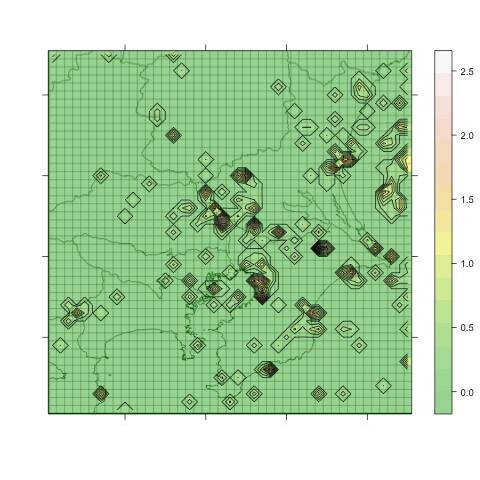
\includegraphics[scale=0.4]{media2010.jpg}
\caption{ GAModel model for the year of 2010.}
\label{modeloGAModel}
\end{figure}

\begin{figure}[H]
\centering
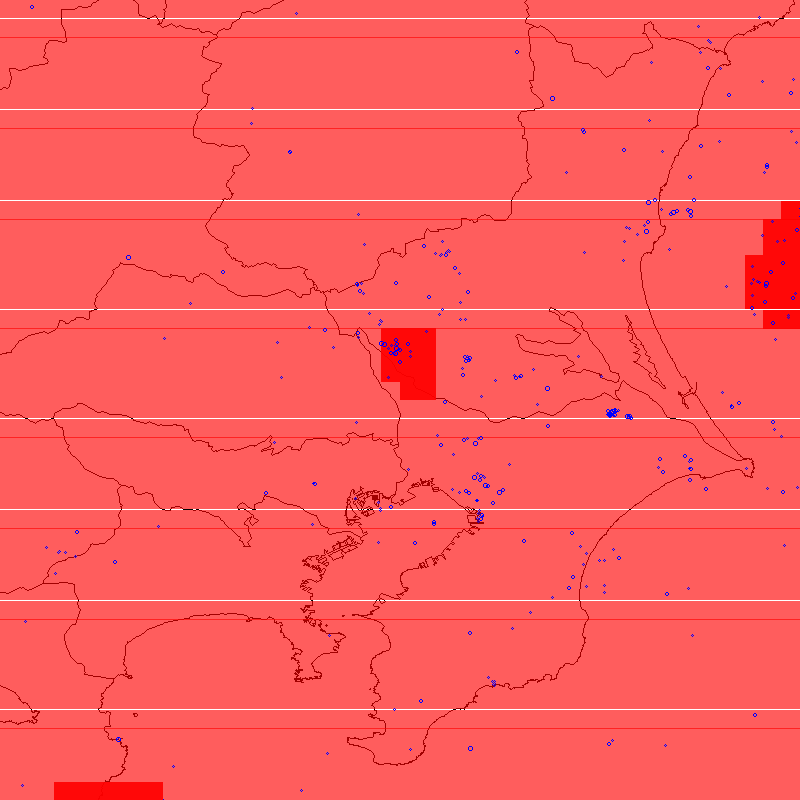
\includegraphics[scale=0.22]{kanto10_RI.png}
\caption{RI model for the year of 2010. Figure from~\cite{ecta14}.}
\label{modeloRI}
\end{figure}

\begin{figure}[H]
\centering
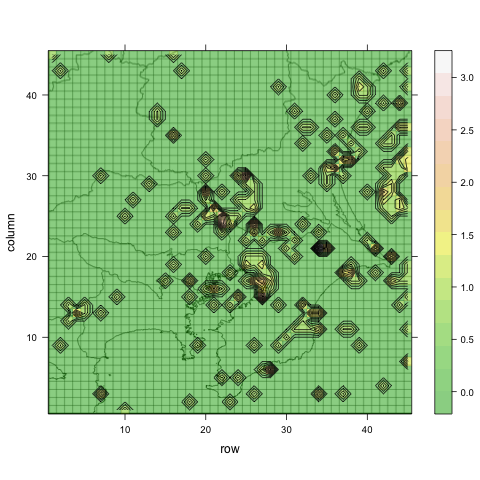
\includegraphics[scale=0.4]{matriz2010_real.png}
\caption{Earthquake occurances for the year of 2010}
\label{realData}
\end{figure}



\section{GAModel X RI Algorithm}
We compared the method proposed, ReducedGAModel,~\ref{ReducedGAModel}, with the non-variated method, GAModel~\ref{GAModel}, and with the Relative Intensity Algorithm,~\ref{ri}, using its log-likelihood values. The values are comparece via Student’s t-test, so we could understand the if there is any statistic significant difference between the methods. The data used was JMA catalog. 


\subsection{Hypothesis}
There are 3 tests hypothesis for this experiment that we want to analyse. 

The first is if the mean values of the log-likelihood for the ReducedGA are equal to the RI values.
$$\begin{cases} H_0: \mu = RI log-likelihood value&\\H_1: \mu != RI log-likelihood value\end{cases}$$

The second is if the mean values of the log-likelihood for the ReducedGA are equal to the GAModel values.
$$\begin{cases} H_0: \mu = GAModel log-likelihood value&\\H_1: \mu != GAModel log-likelihood value\end{cases}$$

And the last hypotheses is if the mean values of the log-likelihood for the GAModel are equal to the RI values.
$$\begin{cases} H_0: \mu = RI log-likelihood value&\\H_1: \mu != RI log-likelihood_value\end{cases}$$

\subsection{Results}

The results of the experiments are in the Table~\ref{gaxriTable} and in the box-plots Figure~\ref{boxPlot2007} and Figure~\ref{boxPlot2009}. The column labeled Random shows the result of the RandomModel, and the idea is the same for the ones labeled GAModel and RI. The ``p-value'' shows the significance value of the {\it Student's t-test} for the null hypothesis `` The mean of the log-likelihood values is greater that the values for RI''.\\

As expected, the RandomModel has lower values than the GAModel. When compared with the RI, the results show that the GAModel is competitive with the RI and that it is promising to use GA to generate earthquake forecasts.\\

\begin{table*}[!ht]
	\begin{center}
		\begin{tabular}{|l|l|c|cc|c|}
			\hline
			\multicolumn{1}{|c|}{Scenario} & \multicolumn{5}{|c|}{Log Likelihood} \\
			\hline
			\multicolumn{1}{|c|}{Year} & \multicolumn{1}{|c|}{Random} & \multicolumn{1}{|c|}{RI} & \multicolumn{2}{c}{GAModel} & \multicolumn{1}{|c|}{p-value} \\    
			%    Ano & Random & RI & GAModel & p-value\\
			\hline
			2000 &-2413.89 &-2124.44 &\raggedright  -2094.05 &\raggedleft (8.80) & 0.01\\%better
			2001 &-2418.14 &-2103.19 &\raggedright  -2101.65 &\raggedleft  (69.49) & 0.57\\%equal
			2002 &-2385.04 &-2094.43 &\raggedright  -2100.01 &\raggedleft (72.62) & 0.07\\%equal
			2003 &-2401.00 &-2104.65 &\raggedright  -2100.76 &\raggedleft (156) & 0.35\\%equal
			2004 &-2421.92 &-2101.92 &\raggedright  -2098.30 &\raggedleft (55.28) & 0.16\\%equal
			2005 &-2643.38 &-2248.40 &\raggedright  -2114.00 &\raggedleft (779) & 0.01\\%better
			2006 &-2616.50 &-2226.93 &\raggedright  -2115.6 &\raggedleft (633) & 0.01\\%better
			2007 &-2451.68 &-2109.13 &\raggedright  -2122.03 &\raggedleft (615) &  0.13\\%equal
			2008 &-2433.23 &-2112.92 &\raggedright  -4435.34 &\raggedleft (657) & 0.14\\%equal
			2009 &-2884.74 &-2438.10 &\raggedright  -2113.1 &\raggedleft (814) & 0.01\\%better
			2010 &-2418.18 &-2114.60 &\raggedright -2112.07 &\raggedleft (843) & 0.79\\%equal
			\hline
		\end{tabular}
	\end{center}
	\caption{Experiments result.}
	\label{gaxriTable}
\end{table*}

\begin{figure}[H]
	\centering
	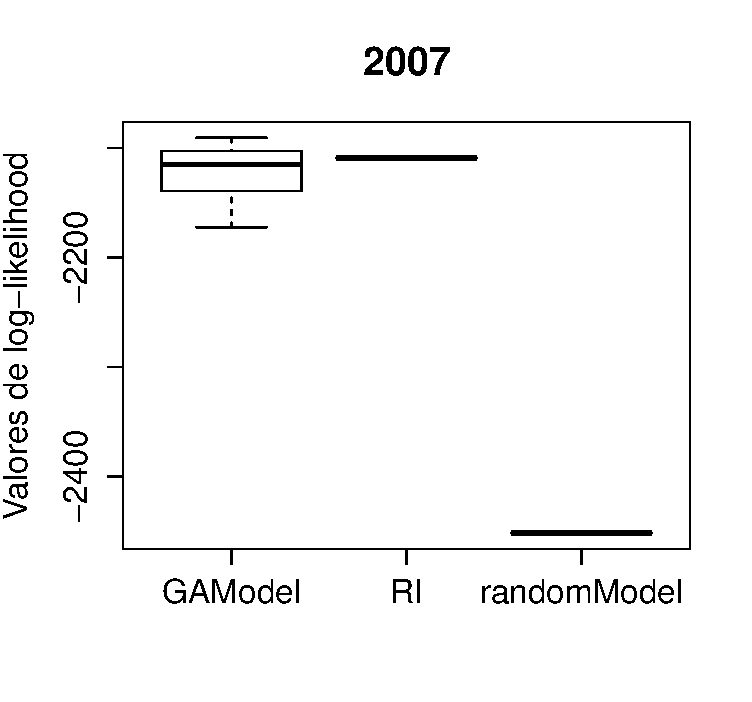
\includegraphics[scale=0.45]{boxPlot2007.pdf}
	\caption{Box-plot of the values obtained by the models for the year 2007.}
	\label{boxPlot2007}
\end{figure}

\begin{figure}[H]
	\centering
	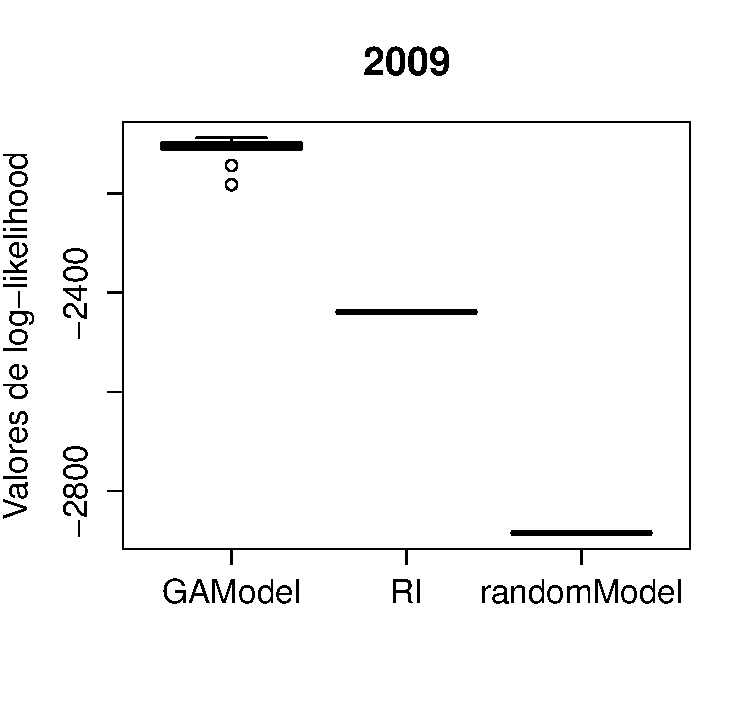
\includegraphics[scale=0.45]{boxPlot2009.pdf}
	\caption{Box-plot of the values obtained by the models for the year 2009.}
	\label{boxPlot2009}
\end{figure}


\section{All Models Experiments}
\subsection{A Brief Recapitulation of the Models}

Based on our promissing results and because we aim to improve them, we developed the ReducedGAModel. It a simplified version of the GAModel. We want to compare the behavior of this new method against the GAModel method.\\

We also wanted to explore how adding domain knowledge would improve the avarage performance of the GAModel or the ReducedGAMOdel. They are versions of GAModel/ReducedGAModel combined with emperical laws.\\ 

\subsection{The Catalogs}

The data used was JMA catalog and a version of a cluster catalog.\\ 
(JMA X métodoJanelaJMA=>clustered). How do I explain this? The EXPLANATION SHOULD BE IN THE FORMER CHAPTER
here is just a recap
\subsection{The Experiment}
For this new experiment, we used even more scenarios (space/time regions) than the ones. Each scenario contains the earthquakes for the regions of Kanto, Kansai, Touhoku and East Japan for a given year (2005-2010). We wanted to explore if there exists any influence in the performance of the models that are caused by the depth of an earthquake. So, the scenarios are also composed by introducing a 3 groups depths thresholds. They are: of earthquakes with depth smaller than 25km, or between 0km and 60km or even between 0km and 100km.\\

These method are stochastic method and hence are variations of the GAModel, we decided to maintain the number of repetitions without redoing a Power Test.\\

\subsection{ANOVA test and HSD Tukey}

The goal here is to find if there is any variation between the methods and which are the most influencial variables. For achieve that, we will use the ANOVA Test.\\

In the ANOVA test, if a variable is out of the 5\% confidence interval, with P < 0.05 it means that there exists a statistical significant different for that variable.\\

There are some tests hypothesis for this experiment that we want to analyse. They all can be generalized as follows:\\

$$\begin{cases} H_0: \text{The population means are equal populacionais são iguais.} &\\
H_1: \text{The population means are different.}&\\
\end{cases}$$\\

Then we apply a post hoc test, the HSD Tukey test, on the results obtained from the ANOVA test to specify which groups differ. \\

\subsection{Results}
A one-way between subjects ANOVA was conducted to compare the effects of the models, the depths, the years and regions on the log-likelihood value. In this study there are 6 options for model: lista, gaModel, hybridgaModel, hybridlist, gaModelCluster and listaCluster. Based on the results of the test, there was a not a significant effect of the depths or years variables. For both cases at the we obtaind p>0.05 level for the depths condition [F(2) = 2.072, p = 0.126] and we also obtained p>0.05 for the years condition  [F(5) = 0.050, p = 0.999]. There was a significant effect of the models condition (p>0.05 [F(5) = 9699.690, p<2e-16]) and regions condition (p>0.05 [F(3) = 764.220, p<2e-16]). Therefore, we conduct a new anova test, with only the last two variables to verify the influence of those conditions more accurately. The results only changed a little, maintaining the significant effect of both conditions, p>0.05 [F(5) = 9705.6, p<2e-16] and p>0.05 [F(3) = 764.7, p <2e-16], respectively.\\

The results of the experiments are in the Table~\ref{anovatest}. 

The column labeled Random shows the result of the RandomModel, and the idea the is same for the ones labeled GAModel and RI.
 means of several groups are equal,e t-test to more than two groups.
 The ``p-value'' shows significance value of the {\it Student's t-test} for null hypothesis `` The mean of the log-likelihood values is greater that the values for RI''.\\

\begin{table*}[!ht]
	\centering
	\begin{tabular}{|l|l|l|l|l|l|}
		\hline
		{Variable} & {Degrees of Freedom} & {Sum Sq}    & {Mean Sq}   & {F Value} & {Pr(\textgreater F)} \\
		\hline
		Model    & 31424058           & 6284812   & 6284812   & 255.0   & \textless2e-16     \\
		\hline
		Depth    & 2                  & 16077491  & 8038746   & 326.2   & \textless2e-16     \\
		\hline
		Year     & 5                  & 57908014  & 11581603  & 470.0   & \textless2e-16     \\
		\hline
		Region   & 3                  & 878253346 & 292751115 & 11879.4 & \textless2e-16\\    
		\hline
	\end{tabular}
	\caption{ANOVA test results.}
	\label{anovatest}
\end{table*}

Because we found statistically significant result, we applied a Post hoc comparisons using the Tukey HSD test. It compared each condition with all others. For example, it compares the values from the gaModel with the gaModelClustered, see~\ref{modelANOVA}. It indicated that the gaModelCluster and ReducedGAModelCluster, when comparared with all other models, achieve greater log-likelihood values. Furthermore, we noticed that the depths conditions show a greater influence when the depth in smaller or equal to 25 km, see Figure~\ref{depthsANOVA}\\

\begin{figure}[H]
	\centering
	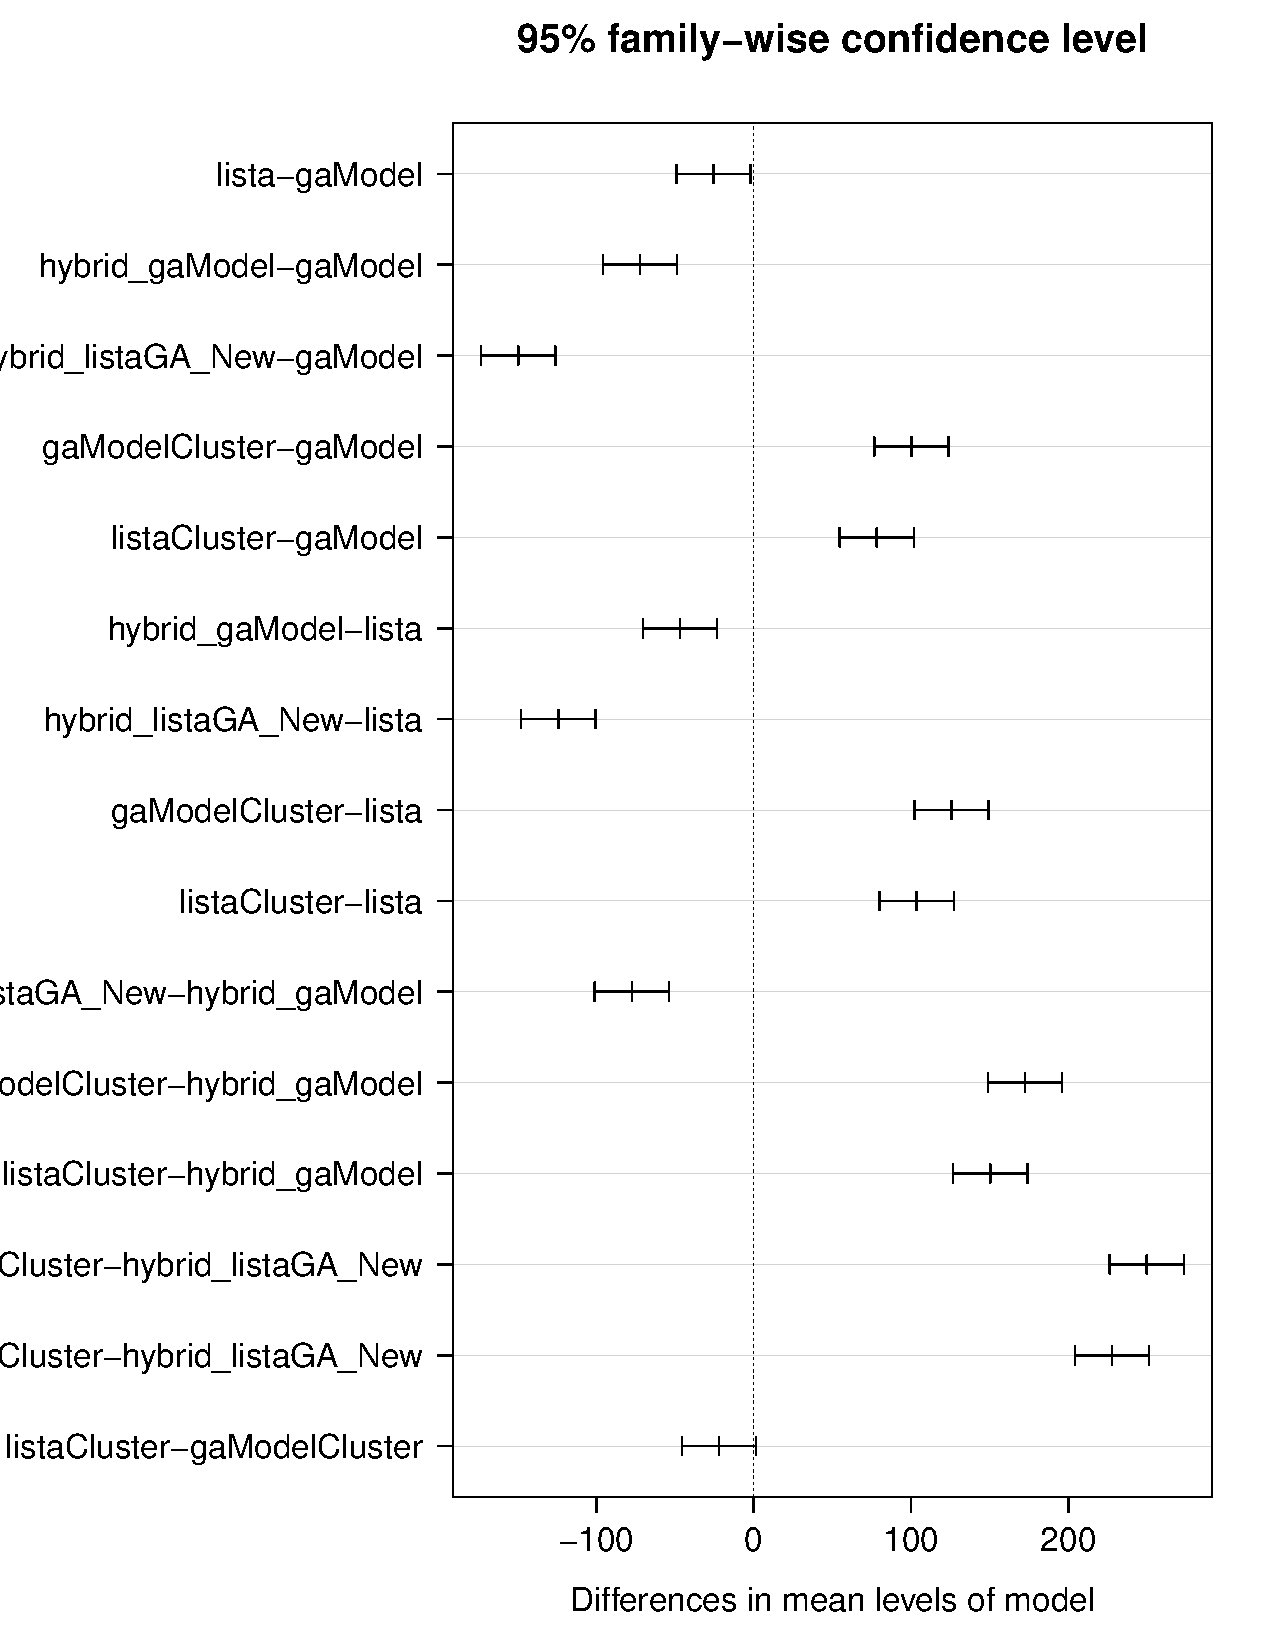
\includegraphics[scale=0.45]{modelANOVA.pdf}
	\caption{.}
	\label{modelANOVA}
\end{figure}

\begin{figure}[H]
	\centering
	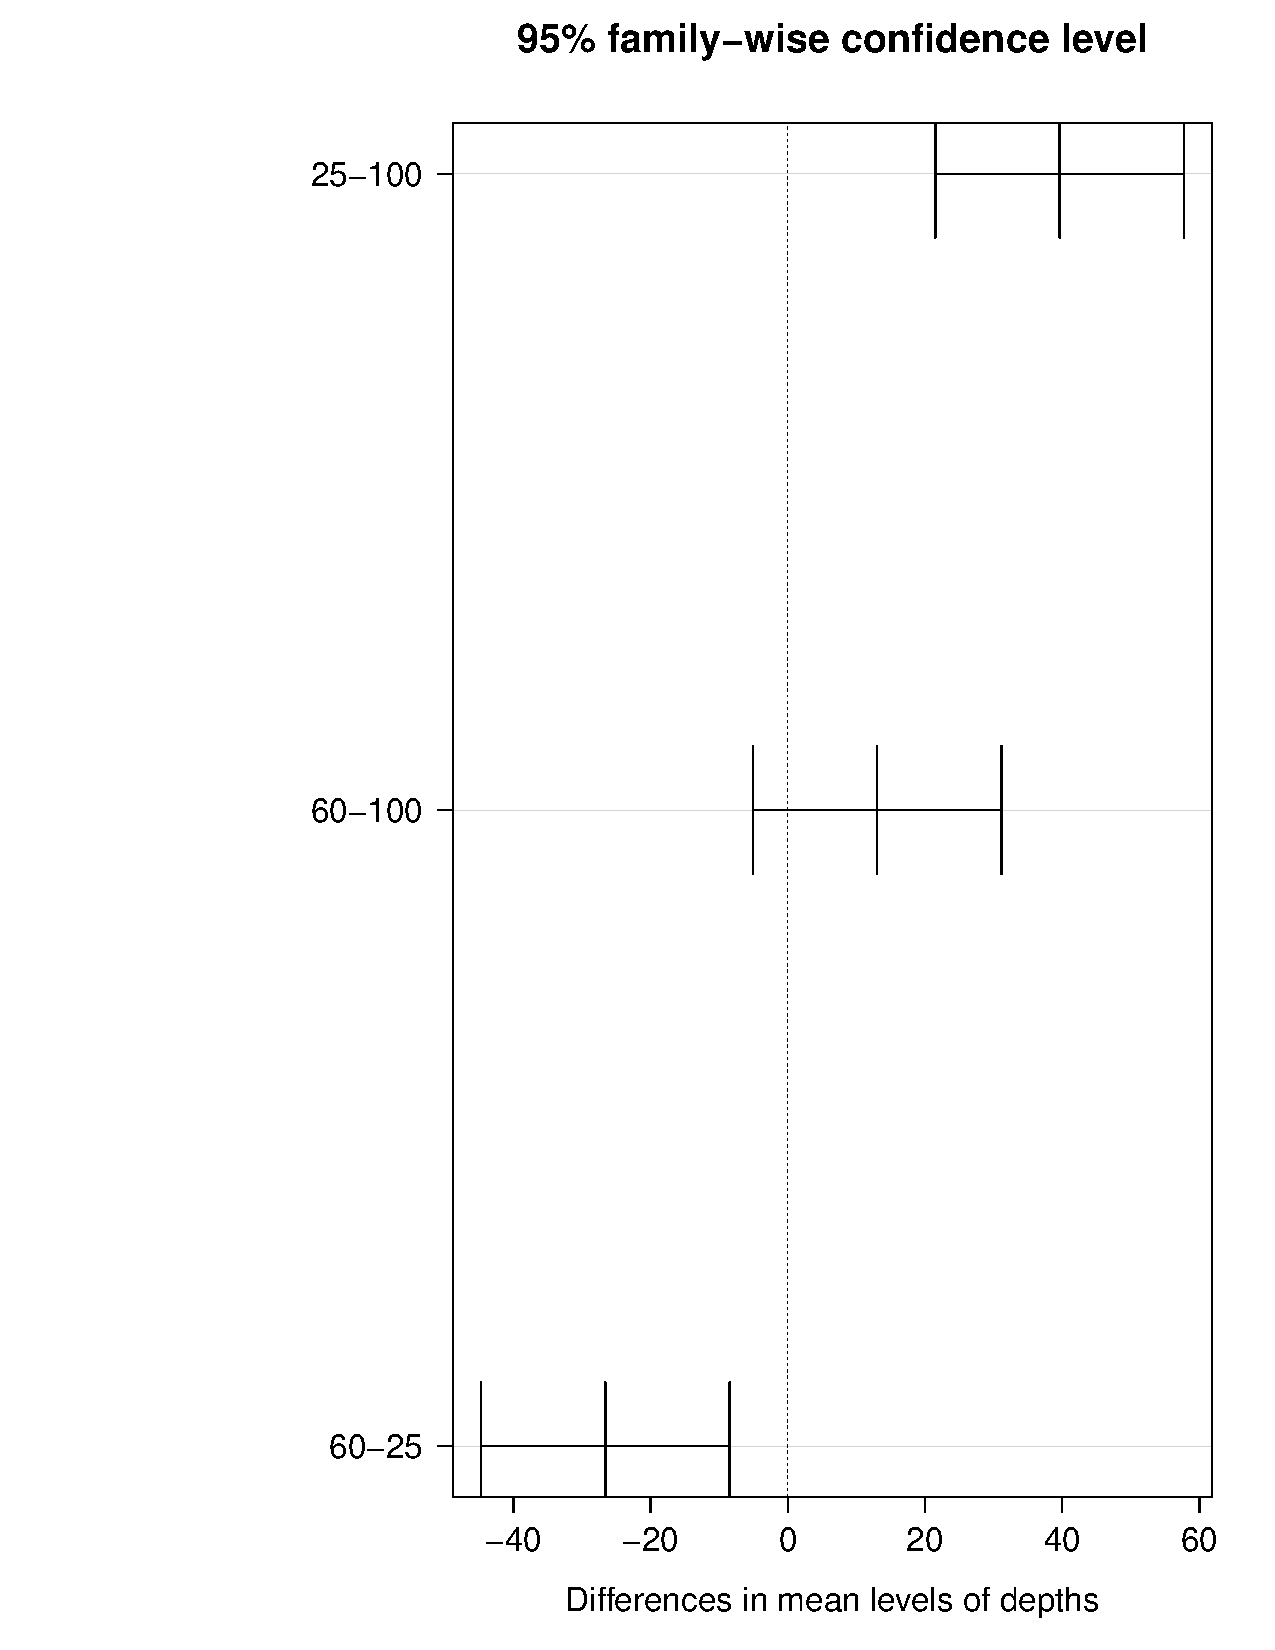
\includegraphics[scale=0.45]{depthsClusterANOVA.pdf}
	\caption{.}
	\label{depthsANOVA}
\end{figure}

When comparing the models from the ReducedGAModel and from the gaModel against themselves, with or without using clustering catalogs, we found that there is no statistically significant result between the methods. That implies it can be considered that the methods are obtain statistically equal results.\\

Therefore, based on the result of HSD test, we performed a new AVOVA test, considering only the gaModelClustered and the listaClustered. That was meant not only to verify the previous results but also to certify if the depth influence is preserved.\\

\begin{table*}[!ht]
	\centering
	\begin{tabular}{|l|l|l|l|l|l|}
		\hline
		{Variable} & {Degrees of Freedom} & {Sum Sq}    & {Mean Sq}   & {F Value} & {Pr(\textgreater F)} \\
		\hline
		Model    & 1           & 174862   & 174862   & 12.22   & \textless0.000488     \\
		\hline
		
		Depth    & 2                  & 391370  & 195685   & 13.67   & \textless1.32e-06     \\
		\hline
		Year     & 5                  & 18810831  & 3762166  & 262.82   & \textless2e-16     \\
		\hline
		Region   & 3                  & 249741769 & 83247256 & 5815.53 & \textless2e-16\\    
		\hline
	\end{tabular}
	\caption{ANOVA test results.}
	\label{anovatest}
\end{table*}


Taken together, these results suggest that the using cluster and depth smaller or equal to 25km, see Figure~\ref{depthsClusterANOVA} showed the best results.\\

\begin{figure}[H]
	\centering
	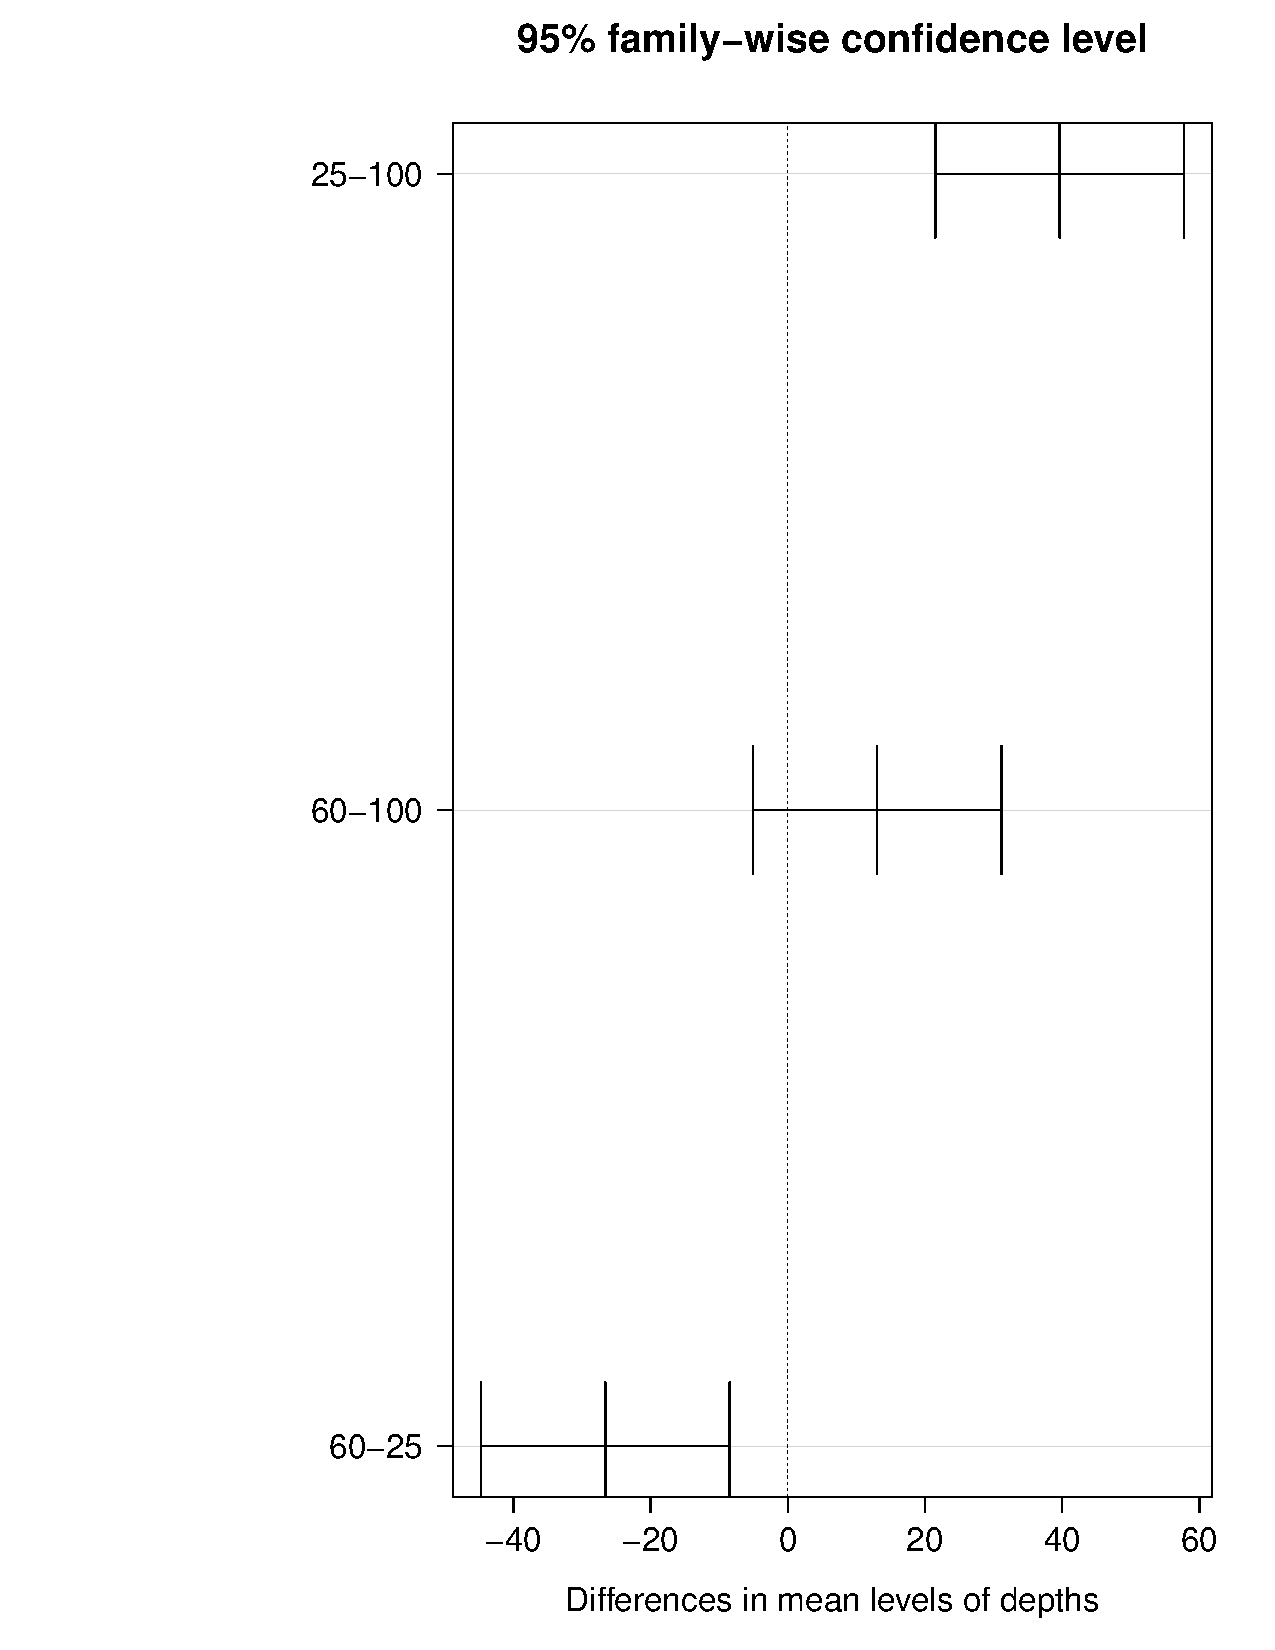
\includegraphics[scale=0.45]{depthsClusterANOVA.pdf}
	\caption{.}
	\label{depthsClusterANOVA}
\end{figure}

\section{Paired Design}

To further explore the only the variations from the models on the regions, disconsidering any other variable, we applied an paired Student’s t-test. 
 tem que fazer isso pra kanto, kansai, touhoku e EastJapan?
%TODO: tem que fazer isso pra kanto, kansai, touhoku e EastJapan?
\begin{table*}[!ht]
	\begin{center}
		\begin{tabular}{|l|l|c|cc|c|}
			\hline
			\multicolumn{1}{|c|}{Scenario} & \multicolumn{5}{|c|}{Log Likelihood} \\
			\hline
			\multicolumn{1}{|c|}{Year} & \multicolumn{1}{|c|}{Random} & \multicolumn{1}{|c|}{RI} & \multicolumn{2}{c}{GAModel} & \multicolumn{1}{|c|}{p-value} \\    
			%    Ano & Random & RI & GAModel & p-value\\
			\hline
			2000 &-2413.89 &-2124.44 &\raggedright  -2094.05 &\raggedleft (8.80) & 0.01\\%better
			2001 &-2418.14 &-2103.19 &\raggedright  -2101.65 &\raggedleft  (69.49) & 0.57\\%equal
			2002 &-2385.04 &-2094.43 &\raggedright  -2100.01 &\raggedleft (72.62) & 0.07\\%equal
			2003 &-2401.00 &-2104.65 &\raggedright  -2100.76 &\raggedleft (156) & 0.35\\%equal
			2004 &-2421.92 &-2101.92 &\raggedright  -2098.30 &\raggedleft (55.28) & 0.16\\%equal
			2005 &-2643.38 &-2248.40 &\raggedright  -2114.00 &\raggedleft (779) & 0.01\\%better
			2006 &-2616.50 &-2226.93 &\raggedright  -2115.6 &\raggedleft (633) & 0.01\\%better
			2007 &-2451.68 &-2109.13 &\raggedright  -2122.03 &\raggedleft (615) &  0.13\\%equal
			2008 &-2433.23 &-2112.92 &\raggedright  -4435.34 &\raggedleft (657) & 0.14\\%equal
			2009 &-2884.74 &-2438.10 &\raggedright  -2113.1 &\raggedleft (814) & 0.01\\%better
			2010 &-2418.18 &-2114.60 &\raggedright -2112.07 &\raggedleft (843) & 0.79\\%equal
			\hline
		\end{tabular}
	\end{center}
	\caption{Experiments result.}
	\label{gaxriTable}
\end{table*}


  
\section{Results from the GAModel Experiment}

The results of the experiments are in the Table~\ref{gaxriTable} and in the box-plots Figure~\ref{boxPlot2007} and Figure~\ref{boxPlot2009}. The column labelled Random shows the result of the RandomModel, and the idea is the same for the ones labelled GAModel and RI. The ``p-value'' shows the significance value of the {\it Student's t-test} for the null hypothesis `` The mean of the log-likelihood values is greater that the values for RI''.\\

As expected, the RandomModel has lower values than the GAModel. When compared with the RI, the results show that the GAModel is competitive with the RI and that it is promising to use GA to generate earthquake forecasts.\\

\begin{table*}[!ht]
	\begin{center}
		\begin{tabular}{|l|l|c|cc|c|}
			\hline
			\multicolumn{1}{|c|}{Scenario} & \multicolumn{5}{|c|}{Log Likelihood} \\
			\hline
			\multicolumn{1}{|c|}{Year} & \multicolumn{1}{|c|}{Random} & \multicolumn{1}{|c|}{RI} & \multicolumn{2}{c}{GAModel} & \multicolumn{1}{|c|}{p-value} \\    
			\hline
			2000 &-2413.89 &-2124.44 &\raggedright  -2094.05 &\raggedleft (8.80) & 0.01\\%better
			2001 &-2418.14 &-2103.19 &\raggedright  -2101.65 &\raggedleft  (69.49) & 0.57\\%equal
			2002 &-2385.04 &-2094.43 &\raggedright  -2100.01 &\raggedleft (72.62) & 0.07\\%equal
			2003 &-2401.00 &-2104.65 &\raggedright  -2100.76 &\raggedleft (156) & 0.35\\%equal
			2004 &-2421.92 &-2101.92 &\raggedright  -2098.30 &\raggedleft (55.28) & 0.16\\%equal
			2005 &-2643.38 &-2248.40 &\raggedright  -2114.00 &\raggedleft (779) & 0.01\\%better
			2006 &-2616.50 &-2226.93 &\raggedright  -2115.6 &\raggedleft (633) & 0.01\\%better
			2007 &-2451.68 &-2109.13 &\raggedright  -2122.03 &\raggedleft (615) &  0.13\\%equal
			2008 &-2433.23 &-2112.92 &\raggedright  -4435.34 &\raggedleft (657) & 0.14\\%equal
			2009 &-2884.74 &-2438.10 &\raggedright  -2113.1 &\raggedleft (814) & 0.01\\%better
			2010 &-2418.18 &-2114.60 &\raggedright -2112.07 &\raggedleft (843) & 0.79\\%equal
			\hline
		\end{tabular}
	\end{center}
	\caption{Experiments result.}
	\label{gaxriTable}
\end{table*}

\begin{figure}[H]
	\centering
	\begin{minipage}{0.45\textwidth}
		\centering
		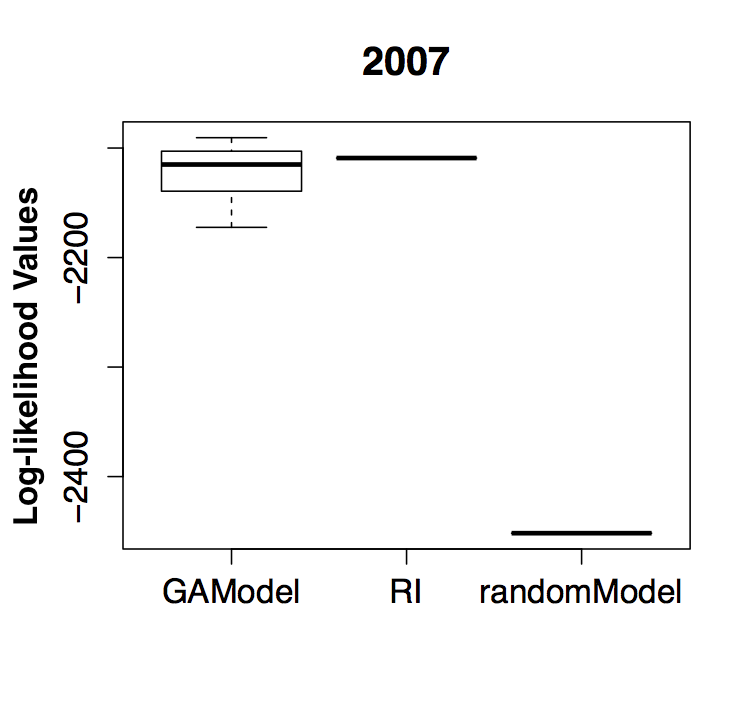
\includegraphics[scale=0.55]{boxPlot2007.png}
		\caption{Box-plot of the values obtained by the models for the year 2007.}
		\label{boxPlot2007}
	\end{minipage}\hfill
	\begin{minipage}{0.45\textwidth}
		\centering
		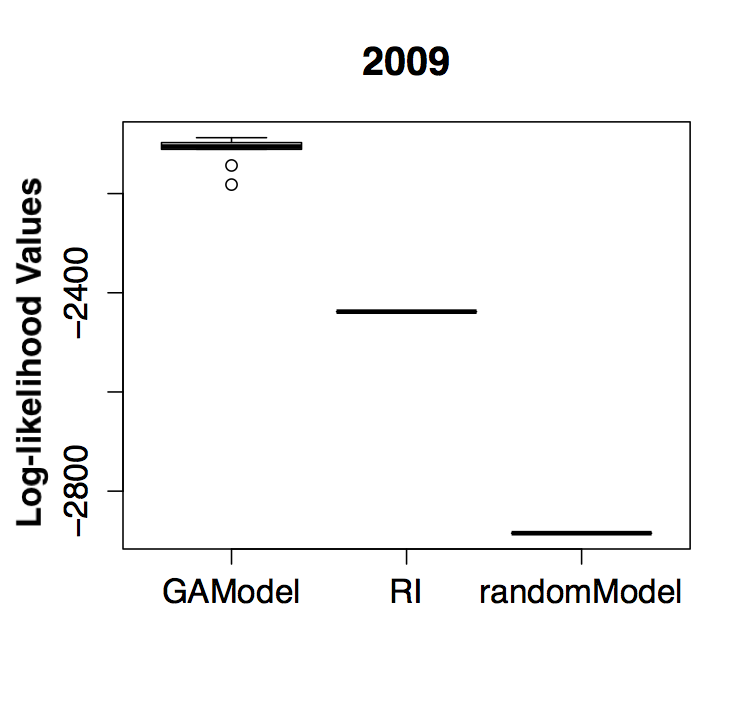
\includegraphics[scale=0.55]{boxPlot2009.png}
		\caption{Box-plot of the values obtained by the models for the year 2009.}
		\label{boxPlot2009}
	\end{minipage}
\end{figure}

\subsection{Models Example and The Real Data}

The Figure~\ref{modeloGAModel} shows a model from the GAModel method for the year 2010. It indicates a low earthquake intensity as green while the more intensity areas, are shown as orange (for even higher cases, white is used). The Figure~\ref{modeloRI} shows a model from the RI Algorithm for the year 2010. It indicates a low earthquake intensity as white while the more intensity areas, are shown in red. For comparison reasons, we show the Figure~\ref{realData}, that shows the earthquake occurrences for the same year.\\


\begin{figure}[H]
	\centering
	\begin{minipage}{0.45\textwidth}
		\centering
		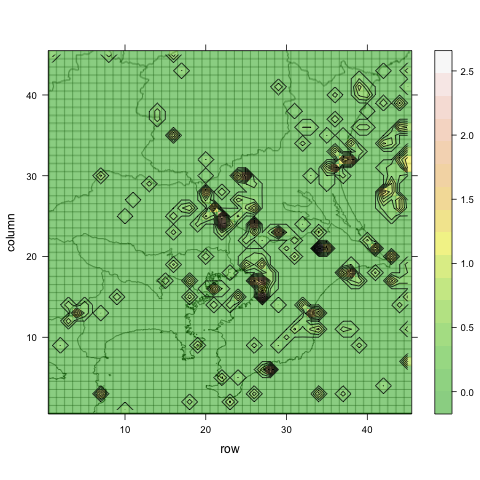
\includegraphics[scale=0.4]{media2010.png}
		\caption{ GAModel model for the year of 2010 in Kanto.}
		\label{modeloGAModel}
	\end{minipage}\hfill
	\begin{minipage}{0.45\textwidth}
		\centering
			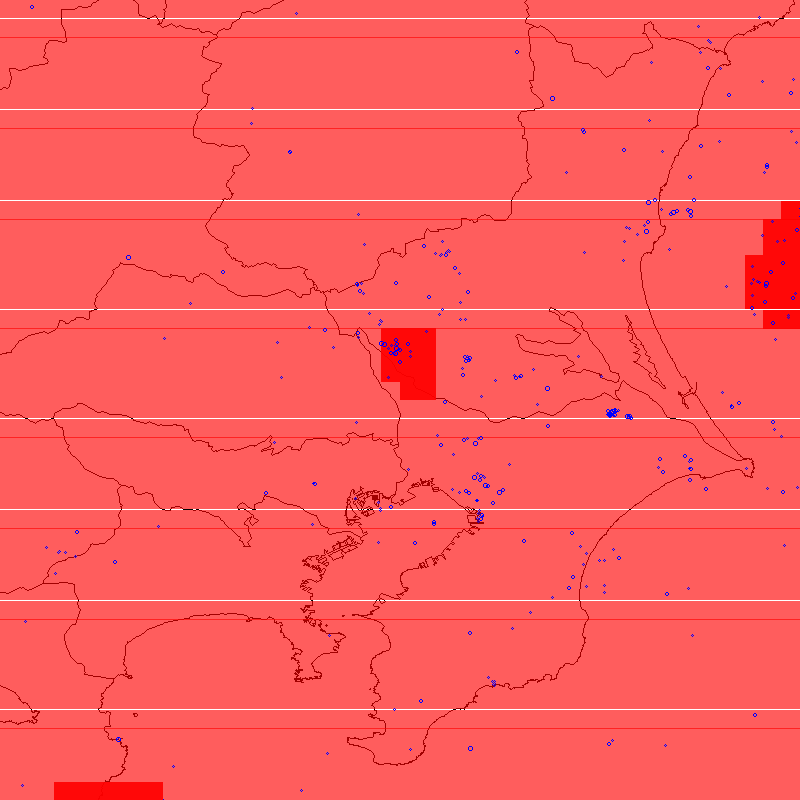
\includegraphics[scale=0.18]{kanto10_RI.png}
			\caption{RI model for the year of 2010 in Kanto. Figure from~\cite{ecta14}.}
			\label{modeloRI}
	\end{minipage}
\end{figure}

\begin{figure}[H]
		\centering
		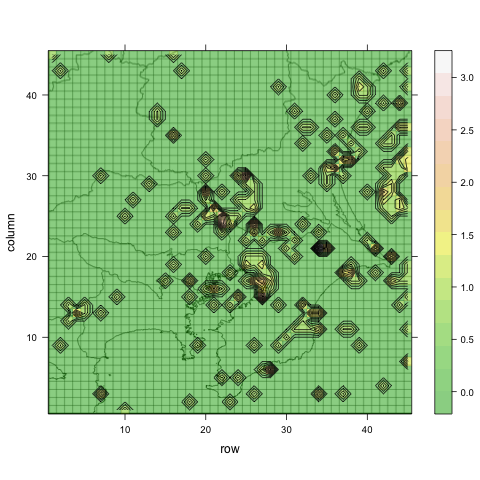
\includegraphics[scale=0.4]{matriz2010_real.png}
		\caption{Earthquake occurrences in the year of 2010 in Kanto.}
		\label{realData}
\end{figure}


\section{Results from The Main-shock Models Main-shock with After-shock Models Experiment}\label{resultsBigExp}

An one-way between subjects ANOVA was conducted to compare the effects of the models, the depths, the years and regions on the log-likelihood value. In this study there are the models: ReducedGAModel, GAModel, Emp-GAModel, Emp-ReducedGAModel, GAModelWindow, ReducedGAModelWindow, GAModelSLC, ReducedGAModelSLC, Emp-GAModelClustered, Emp-ReducedGAModelWindow, Emp-GAModelSLC and Emp-ReducedGAModelSLC.  \\

Based on the results of this first test, it is evident that all variables are significantly different. The results of the experiments are in the Table~\ref{anovatest1}. For all, the confidence interval is set to 5\%.\\

The column labelled Random shows the result of the RandomModel, and the idea the is same for the ones labelled GAModel and RI. The ``p-value'' shows significance value of the {\it Student's t-test} for null hypothesis `` The mean of the log-likelihood values is greater that the values for RI''.\\

\begin{table*}[!ht]
	\centering
	\begin{tabular}{|l|l|l|l|l|l|}
		\hline
		{Variable} & {Degrees of Freedom} & {Sum Sq}    & {Mean Sq}   & {F Value} & {Pr(\textgreater F)} \\
		\hline
		Model    & 11           	  & 1.984e+08  & 18035604   & 113.87    & \textless2e-16     \\
		\hline
		Depth    & 2                  & 2.955e+07  & 14772789   & 93.27     & \textless2e-16     \\
		\hline
		Year     & 5                  & 1.065e+09  & 213025401  & 1344.95   & \textless2e-16     \\
		\hline
		Region   & 3                  & 2.188e+09  & 729443498  & 4605.38   & \textless2e-16	\\    
		\hline
	\end{tabular}
	\caption{Simple ANOVA Test Results.}
	\label{anovatest1}
\end{table*}


Because we found statistically significant result, we applied a Post hoc comparisons using the Tukey HSD test. It compared each condition with all others. For example, it compares the values from the GAModel with the GAModelWindow, see Figure~\ref{modelANOVA}. It indicated that the models that used the catalogues from the Window Method or the Single Link Cluster, when compared with all other models, achieve greater log-likelihood values. Furthermore, we noticed that the depths conditions show a greater influence when the depth in smaller or equal to 25 km, see Figure~\ref{depthsANOVA}.\\

\begin{figure}[H]
	\centering
	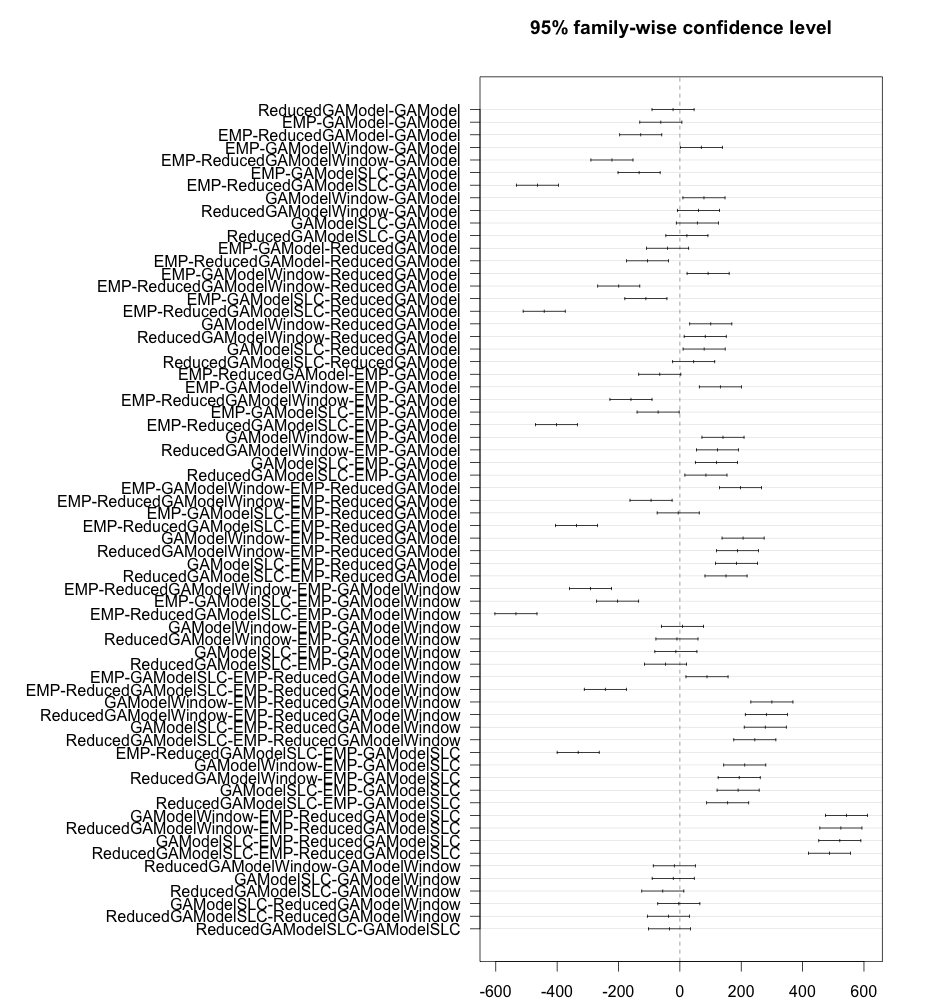
\includegraphics[scale=0.45]{1modelANOVA.png}
	\caption{ANOVA results - Models.}
	\label{modelANOVA}
\end{figure}

\begin{figure}[H]
	\centering
	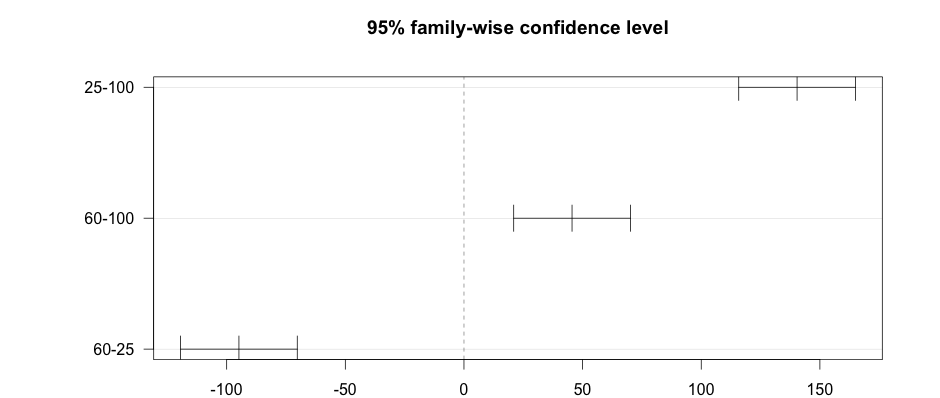
\includegraphics[scale=0.45]{depthsClusterANOVA.png}
	\caption{ANOVA results - Depths.}
	\label{depthsANOVA}
\end{figure}

Then, we decided to compare only the those models against themselves. That is, models used for this new comparison are those that used the catalogues from the Window Method or the Single Link Cluster and with earthquakes with depth smaller or equal to 25 km.\\

\begin{table*}[!ht]
	\centering
	\begin{tabular}{|l|l|l|l|l|l|}
		\hline
		{Variable} & {Degrees of Freedom} & {Sum Sq}    & {Mean Sq}   & {F Value} & {Pr(\textgreater F)} \\
		\hline
		Model    & 7            	  & 21991488   & 3141641    & 21.07     & \textless2e-16     \\
		\hline
		Year     & 5                  & 240753808  & 48150762   & 322.94    & \textless2e-16     \\
		\hline
		Region   & 3                  & 374602684  & 124867561  & 837.48    & \textless2e-16	\\    
		\hline
	\end{tabular}
	\caption{Simple ANOVA Test Results.}
	\label{anovatest2}
\end{table*}

Based on the results of this test, it is evident that all variables are still significantly different. The results of the experiments are in the Table~\ref{anovatest2}. For all, as before, the confidence interval is set to 5\%.\\


Again, we found statistically significant result, therefore, we applied the Tukey HSD test. The results are shown in Figure~\ref{modelANOVA2}. It indicated that the models from the GAModel method, when compared with all other models, achieve greater log-likelihood values.\\

\begin{figure}[H]
	\centering
	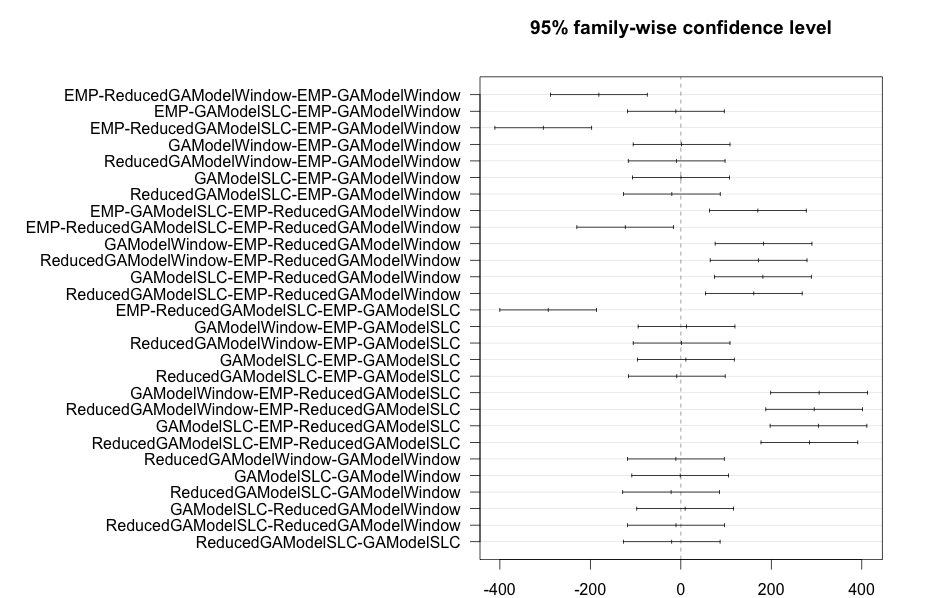
\includegraphics[scale=0.45]{2modelANOVA.png}
	\caption{ANOVA results - Models.}
	\label{modelANOVA2}
\end{figure}

Based on the last results, we performed the ANOVA again, comparing only models from the GAModel method. The results of the experiments are in the Table~\ref{anovatest3}.\\

\begin{table*}[!ht]
	\centering
	\begin{tabular}{|l|l|l|l|l|l|}
		\hline
		{Variable} & {Degrees of Freedom} & {Sum Sq}    & {Mean Sq}   & {F Value} & {Pr(\textgreater F)} \\
		\hline
		Model    & 3            	  & 24462      & 8154       & 0.058      &  0.981      \\
		\hline
		Year     & 5                  & 121287074  & 24257415   & 173.600    & \textless2e-16     \\
		\hline
		Region   & 3                  & 167719464  & 55906488   & 400.099    & \textless2e-16	\\    
		\hline
	\end{tabular}
	\caption{Simple ANOVA Test Results.}
	\label{anovatest3}
\end{table*}

This time, we found statistically significant result only for the year and region condition. To show that the models results are not statistically different from each other, we applied a pairing analysis.\\

From the the pairing analysis, we decided to use the \textit{GAModelWindow} as the representative method of this study. That is because, in most cases when its values were compared, it showed a little better performance in the means of the log-likelihood values. For the results, see the Table~\ref{Paired}.\\

\begin{table*}[!ht]
	\begin{center}
		\begin{tabular}{|l|l|c|cc|c|}
			\hline
			\multicolumn{1}{|c|}{Scenario} & \multicolumn{5}{|c|}{Log Likelihood} \\
			\hline
			\multicolumn{1}{|c|}{Models} & \multicolumn{1}{|c|}{Kansai} & \multicolumn{1}{|c|}{Touhoku} & \multicolumn{2}{c}{East Japan} & \multicolumn{1}{|c|}{Kanto} \\    
			\hline
			EMP-GAModelWindow &-2643.38 &-2248.40 &\raggedright  -2114.00 &\raggedleft (779) & 0.01\\%better
			2006 &-2616.50 &-2226.93 &\raggedright  -2115.6 &\raggedleft (633) & 0.01\\%better
			2007 &-2451.68 &-2109.13 &\raggedright  -2122.03 &\raggedleft (615) &  0.13\\%equal
			2008 &-2433.23 &-2112.92 &\raggedright  -4435.34 &\raggedleft (657) & 0.14\\%equal
			2009 &-2884.74 &-2438.10 &\raggedright  -2113.1 &\raggedleft (814) & 0.01\\%better
			2010 &-2418.18 &-2114.60 &\raggedright -2112.07 &\raggedleft (843) & 0.79\\%equal
			\hline
		\end{tabular}
	\end{center}
	\caption{Experiments result.}
	\label{Paired}
\end{table*}


%TODO: add ALL figures
\subsection{The Models Examples And The Real Data}

The Figure~\ref{gamodel2005eastjapan} shows a model from the GAModel method for the year 2005 in East Japan. The next Figure,~\ref{reduced2005eastjapan} shows a model from the ReducedGAModel~\ref{reducedGAModel} method for the year 2005 in East Japan.\\

All Figures,~\ref{gamodel2005eastjapan}~\ref{reduced2005eastjapan}~\ref{hybridgamodel2005eastjapan}~\ref{hybridreduced2005eastjapan},  indicate a low earthquake intensity as white while the more intensity areas, are shown in red. They are, in order, the data visualisation for the model from: the GAModel, the ReducedGAModel, the Emp-GAModel and the Emp-ReducedGAModel for East Japan in 2005. The Figure~\ref{real2005eastjapan} represents the earthquake occurrences in the same region and year.\\


\begin{figure}[H]
		\centering
		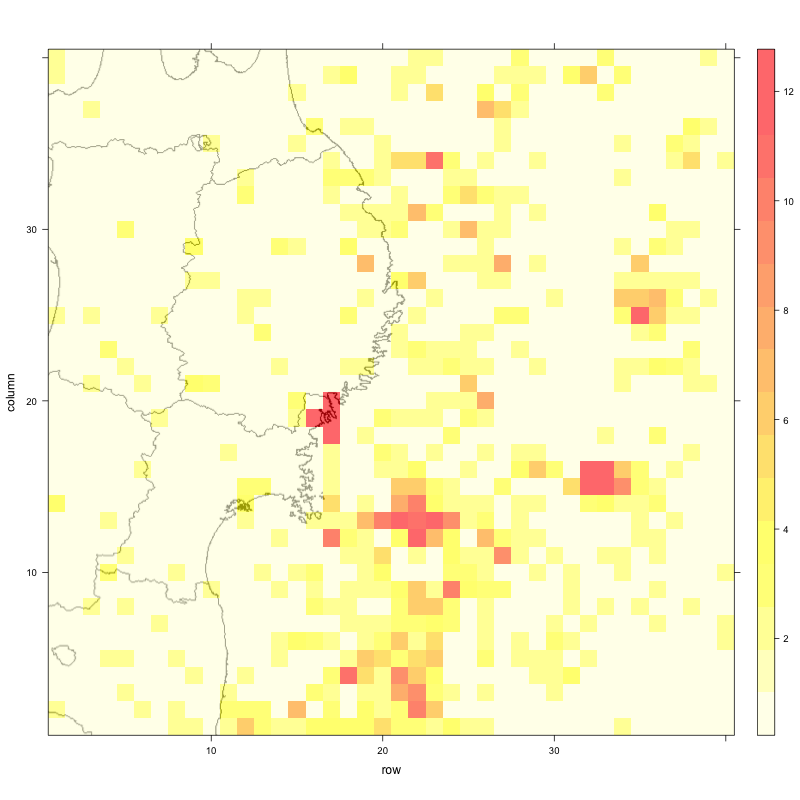
\includegraphics[scale=0.2]{real2005eastjapan.png}
		\caption{Earthquake occurrences in the year of 2005 in East Japan.}
		\label{real2005eastjapan}
\end{figure}


\begin{figure}[H]
	\centering
	\begin{minipage}{0.45\textwidth}
		\centering
		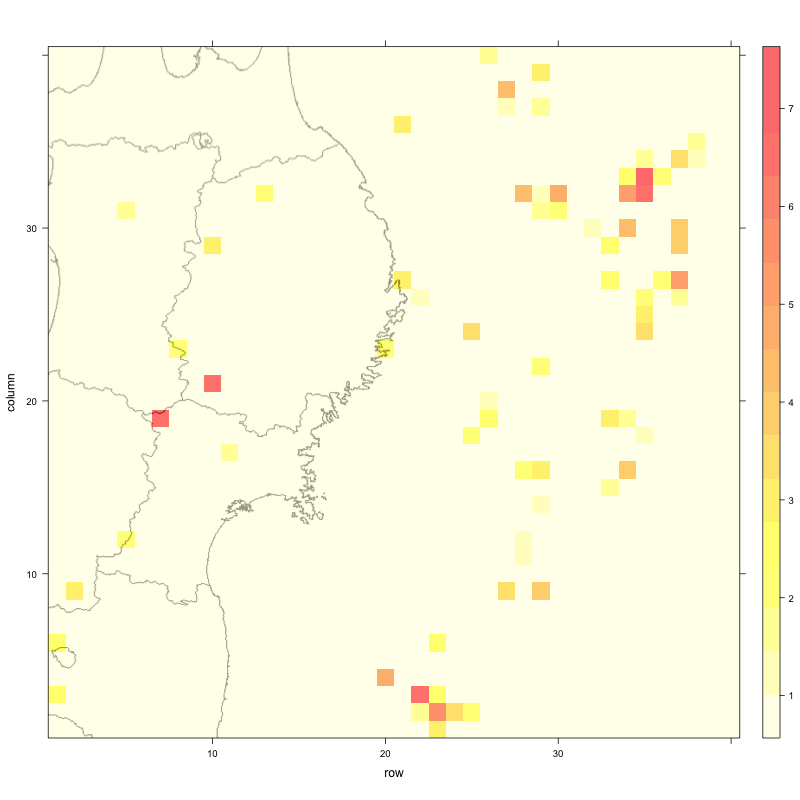
\includegraphics[scale=0.2]{reduced2005eastjapan.png}
		\caption{ReducedGAModel model - year of 2005, East Japan.}
		\label{reduced2005eastjapan}
	\end{minipage}
	\begin{minipage}{0.45\textwidth}
		\centering
		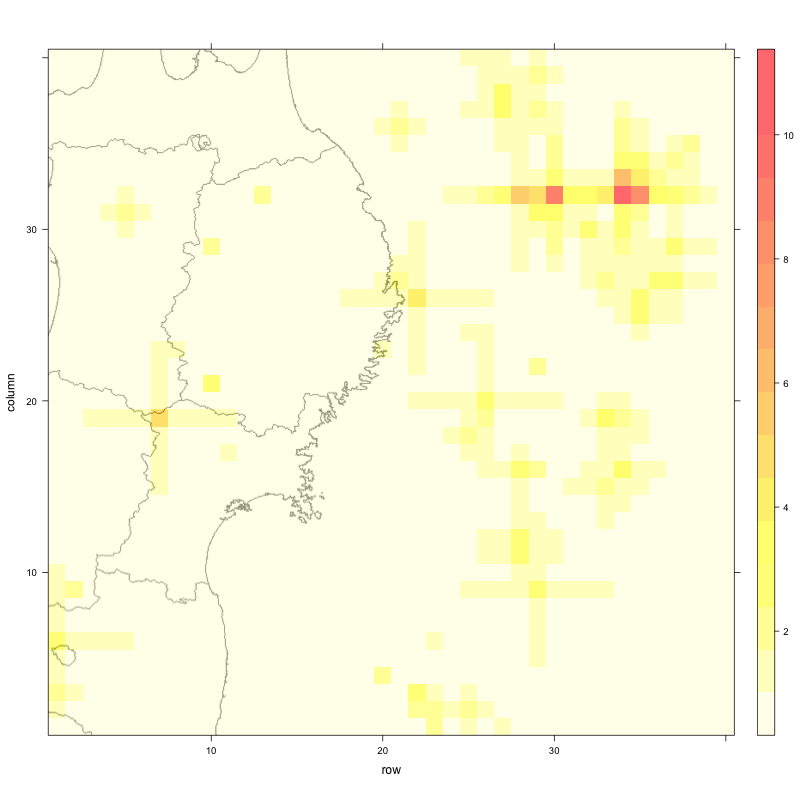
\includegraphics[scale=0.2]{hybridgamodel2005eastjapan.png}
		\caption{Em-GAModel model - year of 2005, East Japan.}
		\label{hybridgamodel2005eastjapan}
	\end{minipage}
\end{figure}

\begin{figure}[H]
	\begin{minipage}{0.45\textwidth}
		\centering
			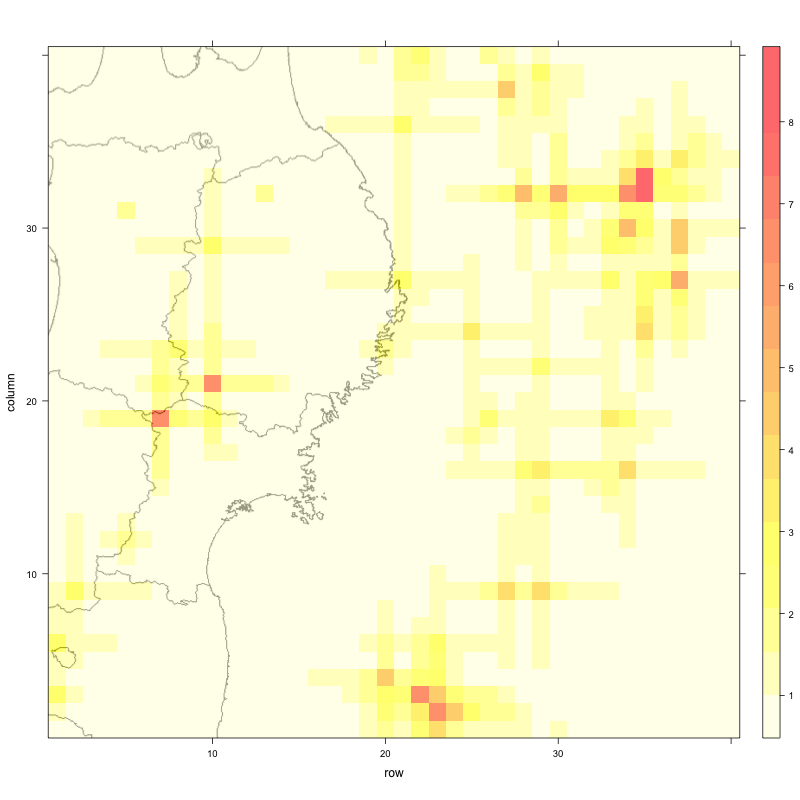
\includegraphics[scale=0.2]{hybridreduced2005eastjapan.png}
			\caption{Emp-ReducedGAModel model - year of 2005, East Japan.}
			\label{hybridreduced2005eastjapan}
	\end{minipage}
	\begin{minipage}{0.45\textwidth}
		\centering
		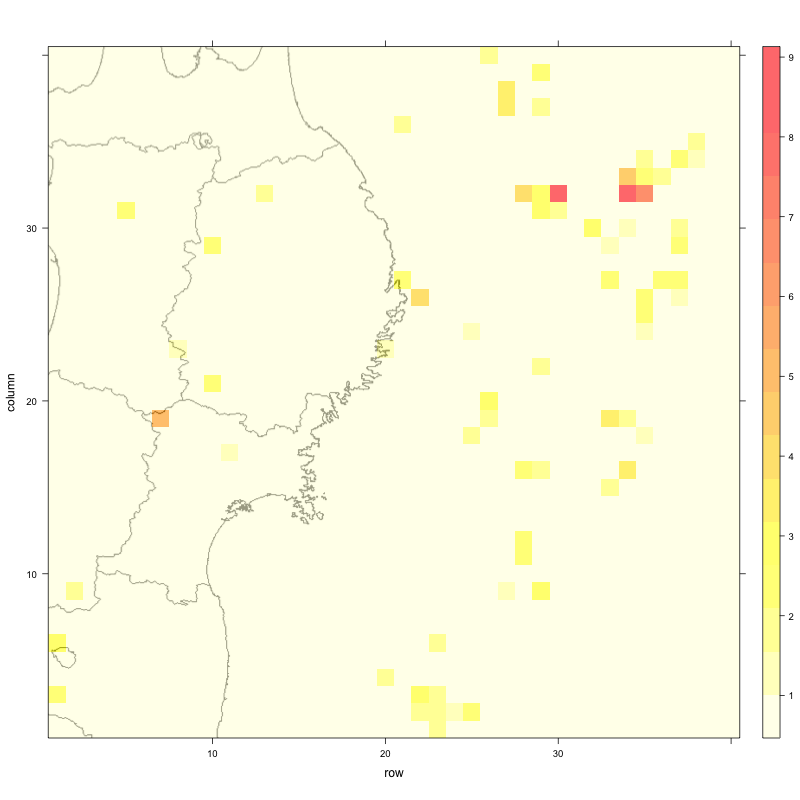
\includegraphics[scale=0.2]{gamodel2005eastjapan.png}
		\caption{GAModel model - year of 2005, East Japan.}
		\label{gamodel2005eastjapan}
	\end{minipage}
\end{figure}

%TODO: add magnitude study!
\section{Magnitude Study}
From the results already obtain and showed in the section~\ref{resultsBigExp}, when selected the models with earthquakes with depth smaller or equal to 25 km and then we split the models in magnitude intervals, as defined in~\ref{magExp}.\\

After that, we compared those split models against themselves. Based on the results of this test, it is evident that all variables are still significantly different. The results of the experiments are in the Table~\ref{anovatestMag}. For all, as before, the confidence interval is set to 5\%.\\

\begin{table*}[!ht]
	\centering
	\begin{tabular}{|l|l|l|l|l|l|}
		\hline
		{Variable} & {Degrees of Freedom} & {Sum Sq}    & {Mean Sq}   & {F Value} & {Pr(\textgreater F)} \\
		\hline
		Model       & 5            	  & 2.368e+09      & 4.737e+08    & 3058     & \textless2e-16     \\
		\hline
		Year        & 3                  & 4.139e+09   & 1.380e+09    & 8906     & \textless2e-16     \\
		\hline
		Magnitude   & 7                  & 3.212e+09   & 4.588e+08    & 2962     & \textless2e-16	\\    
		\hline
	\end{tabular}
	\caption{Simple ANOVA Test Results.}
	\label{anovatestMag}
\end{table*}

We found statistically significant result and, as before, we applied the Tukey HSD test. The results are shown in Figure~\ref{modelANOVAMag} and the \textit{NULL} field was used as the model with all magnitude intervals (the complete model).\\

It indicated that the interval $[3.0-4.0]$ always performed, in terms of log-likelihood values, worse than all other intervals. this phenomenon also happens in the interval $[4.0-5.0]$, though in this case, the difference is not as big as the last one. The other intervals show no significant difference.\\

From the results found, we decided to chose only earthquakes with magnitude higher than 4.0 as our threshold value.\\

\begin{figure}[H]
	\centering
	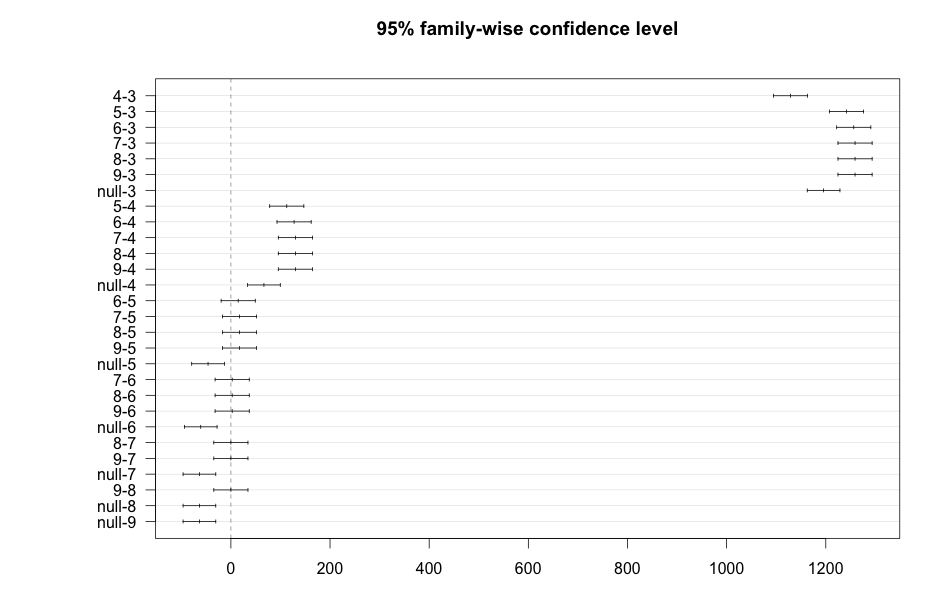
\includegraphics[scale=0.45]{magModels.png}
	\caption{ANOVA results - Models.}
	\label{modelANOVAMag}
\end{figure}



%magModels.png,magyears.png, magRegions.png
  %TODO: add contribuitions and future works
\chapter{Conclusão}\label{chapter8}
Este projeto apresentou uma proposta de desenvolvimento de um modelo de previsão de probabilidades elaborado a partir de uma implementação simples de algoritmos genéticos. Foi possível perceber uma evolução do modelo em relação ao modelo completamente aleatório, caracterizado pela população inicial.\\

Foram muitos os desafios enfrentados ao utilizar os testes propostos pelo RELM como função de {\it fitness} pelo algoritmo genético. O primeiro está relacionada ao tempo de execução e o uso desses a cada geração como função de {\it fitness}. Por se tratar de testes com uma grande quantidade de cálculos em grande quantidades de observações, o tempo gasto para analisar as informações poderia ser demasiado grande para ser viável continuar a utilizar os testes junto ao algoritmo. O segundo problema estava vinculado ao comportamento desses testes em uma aplicação de algoritmos genéticos, pois não havia conhecimento anterior sobre a aplicabilidade desses com Computação Evolutiva e se aplicável, se o resultado seria promissor.\\

Pelos resultados finais do L-test, foi verificado que tanto o primeiro desafio quanto o segundo, não foram suficientes para impossibilitar o uso dos testes e que as gerações de populações resultaram em indivíduos mais aptos para a previsão de sismos. Pelos resultados mostrados o trabalho mostra que aplicar Computação Evolutiva para prever ocorrências de sismos é minimamente promissor, uma vez que há uma evolução do modelo em relação ao modelo pseudo-aleatório.\\

Foi possível, portanto, vincular os testes proposto pelo RELM com algoritmos genéticos. A partir disso, agora, deve-se explorar as características da aplicação, tornar os testes implementados mais completos e estruturados, definir os operadores genéticos visando um comportamento adequado em relação aos indivíduos como para as populações evoluídas.\\

Posteriormente, o primeiro desafio foi minimizado, pelo uso de uma tabela em memória do fatorial. Alguns estudos deverão ser realizados para compreendermos melhor o porquê da alteração dos valores após a introdução da tabela.\\

O uso de operadores de peso adaptativos mostrou-se interessante e é provável que, sua inclusão na GA estudada traga ainda mais benefícios assim que outros problemas forem resolvidos. Problemas, tais quais, a independência dos {\it bins}, que influenciaram negativamente a performance da aplicação e serão alvos de maiores esforços.\\



Algumas propostas de melhorias e trabalhos futuros podem ser listadas:\\

• Compará-lo com um outro modelo de previsão de terremotos, como por exemplo, o {\it Relative Intensity} (RI). Para melhores efeitos de comparação, é interessante acrescentar cálculos de confiabilidade estatísca, como {\it p-value}, e criar um mapa demonstrativo da previsão relativa de cada área representada pelos {\it bins};\\%acho que tem no artigo 

• Implementar o operador de mutação específico para números reais e que tenha um comportamento direcionado a aplicação, capaz de alterar seus valores no decorrer das gerações capaz de equilibrar {\it explotaition} e {\it exploration};\\

• Aplicar alguns testes sugeridos por Zechar\citep{zechartheme} afim de definir a qualidade do modelo desenvolvido;\\

• Fazer analises de complexidade do algoritmo executado;\\

• Criar múltiplas observações para cada indivíduo para que o cálculo de incertezas possa ser aplicado e, assim, aumentarmos a qualidade dos modelos;\\

• Realizar experimentos em outras áreas do Japão, além de Kanto;\\

• Especializar a abordagem de algoritmo genético ({\it crossover} mais apropriado, mutação específica, ...) ou  utilizar soluções híbridas, entre algoritmo genéticos e outras técnicas de aprendizado de máquina;\\

• Incrementar os cálculos estatísticos com as ferramentas adequadas, desvio padrão, variância, etc, que compõe os cálculos dos testes demonstrados;\\

• A fim de evitar o {\it over fitting}, podemos inserir dados sismológicos, como sobre de magnitude e hora da ocorrência, aumentando a área de busca da aplicação;\\

• Cada {\it bin} é trato e considerado individualmente. Portanto a ocorrência de sismos em um {\it bin} não influência ocorrências de sismos em seus vizinhos, o que sabemos não ser verdade;\\

• Contrariando expectativas, execuções com operadores reais obtiveram desempenho pior que com operadores tradicionais pode estar relacionado ao fato de não existir influência entre os {\it bins}, uma vez que pode haver áreas de altíssima probabilidade próximas a áreas de baixa probabilidade.\\

  % ...

  \nocite{*}
  \postextual
  \bibliographystyle{plain}
  \bibliography{bibliografia}

\end{document}
